%!TEX TS-program = pdflatexmk
%this will be based on the amsart class, which probably causes more pain than necessary
%but gets a lot of the formatting the way I like it
%look for !!!EDIT comments
\documentclass[oneside,12pt]{amsart}
\usepackage{amsaddr}
\usepackage[T1]{fontenc}
\usepackage{amsmath,amsfonts,amsthm,amssymb} %provides all math symbols etc.

%graphics
\usepackage{graphicx}
\usepackage{wrapfig}
\usepackage[margin=0.1cm,textfont=it]{caption}

%set 1" margins:
\usepackage[left=1in,top=1in,right=1in,bottom=1in,footskip = 0.333in]{geometry}

%provide additional table capability
\usepackage{tabularx}
\newcolumntype{L}[1]{>{\raggedright\let\newline\\\arraybackslash\hspace{0pt}}m{#1}} %define left justified column type

%pdf handling (only needed if including PDFs)
%\usepackage{pdflscape} 
%\usepackage{rotating}
\usepackage{pdfpages}

%provides nice verbatim environment and allows verbatim in footnotes
%uncomment as needed
%\usepackage{fancyvrb} 

%control enumerate/itemize spacing
\usepackage{enumitem} 

%for editing phase only:
%\usepackage{todonotes}
%\usepackage{draftwatermark}
%\SetWatermarkText{DRAFT}
%\SetWatermarkScale{5}

%no reason spacing should be anything other than single
%\renewcommand{\baselinestretch}{1}\normalsize %single spaced

%set up header (this has to come before the section patching)
\usepackage{fancyhdr}
\setlength{\headheight}{0.2in}
\pagestyle{fancy}
\fancyhf{}
\lhead{\small \sc Program} %!!!EDIT
\chead{\small \sc \rightmark}
\rhead{\footnotesize \thepage}
\renewcommand{\headrulewidth}{0pt}

% need to redefine section to allow rightmark to work with amsart
\let\origsection\section
\renewcommand{\section}[1]{\sectionmark{#1}\origsection{#1}}
% redefine sectionmark
\renewcommand\sectionmark[1]{\markboth{#1}{#1}}

%fix toc
\setcounter{tocdepth}{3}% to get subsubsections in toc
\makeatletter
\renewcommand{\@pnumwidth}{2em}% default is 1.55em -accommodates wider page numbers
\def\@tocline#1#2#3#4#5#6#7{\relax
  \ifnum #1>\c@tocdepth % then omit
  \else
    \par \addpenalty\@secpenalty\addvspace{#2}%
    \begingroup \hyphenpenalty\@M
    \@ifempty{#4}{%
      \@tempdima\csname r@tocindent\number#1\endcsname\relax
    }{%
      \@tempdima#4\relax
    }%
    \parindent\z@ \leftskip#3\relax \advance\leftskip\@tempdima\relax
    \rightskip\@pnumwidth plus4em \parfillskip-\@pnumwidth
    #5\leavevmode\hskip-\@tempdima
      \ifcase #1
       \or\or \hskip 1em \or \hskip 2em \else \hskip 3em \fi%
      #6\nobreak\relax
    \dotfill\hbox to\@pnumwidth{\@tocpagenum{#7}}\par
    \nobreak
    \endgroup
  \fi}
\makeatother

%section numbering
\renewcommand{\thesubsection}{\alph{subsection}}
\renewcommand{\thesubsubsection}{\roman{subsubsection}}
\makeatletter
\renewcommand{\p@subsection}{\thesection.}
\renewcommand{\p@subsubsection}{\thesection.\thesubsection.}
\makeatother

%Define invisible section and subsection for including PDF docs
\newcommand\invisiblesection[1]{%
  \refstepcounter{section}%
  \refstepcounter{page}  %%only if numbering pages within sections
  \addcontentsline{toc}{section}{\protect{\thesection.}{\hskip 1em}#1}%
  \sectionmark{#1}}
  
\newcommand\invisiblesubsection[1]{%
  \refstepcounter{subsection}%
  \addcontentsline{toc}{subsection}{\thesubsection.{\hskip 1em}#1}%
  }
  
%page numbering by section
\numberwithin{page}{section}
\renewcommand{\thepage}{\thesection-\arabic{page}}

%% Make sure that page starts from 1 with every \section
\usepackage{etoolbox}
\makeatletter
\patchcmd{\@sect}% <cmd>
  {\protected@edef}% <search>
  {\def\arg{#1}\def\arg@{section}%
   \ifx\arg\arg@\stepcounter{page}\fi%
   \protected@edef}% <replace>
  {}{}% <success><failure>
\makeatother

%hyperref load has to come after section  patching
\usepackage[breaklinks=true,colorlinks=true,citecolor=red]{hyperref}
\newcommand{\nlhref}[1]{\href{#1}{\nolinkurl{#1}}} %automatically create exact url with href

%create boolean for toggling inclusion of backmatter
\providetoggle{backmatter}
\settoggle{backmatter}{false} %set to true to toggle on/false off %!!!EDIT

%bibliography handling
\usepackage[citestyle=authoryear-comp,bibstyle=numeric, natbib=true, backend=bibtex,hyperref=true,maxbibnames=99,maxcitenames=2]{biblatex}
\addbibresource{Main.bib} %!!!EDIT

% private defs
\def\mf{\mathbf}
\def\mb{\mathbb}
\def\mc{\mathcal}
\newcommand{\bbar}[1]{\mf{\bar{#1}}}
\newcommand{\bhat}[1]{\mf{\hat{#1}}}
\newcommand{\refeq}[1]{Equation  (\ref{#1})}
\newcommand{\refsec}[1]{\S\ref{#1}} 
\newcommand{\reftable}[1]{Table \ref{#1}} 
\newcommand{\refch}[1]{Chapter  \ref{#1}} 
\newcommand{\reffig}[1]{Figure \ref{#1}}
\newcommand{\refcode}[1]{Listing \ref{#1}}
\newcommand{\intd}[1]{\ensuremath{\,\mathrm{d}#1}}
\newcommand{\leftexp}[2]{{\vphantom{#2}}^{#1}\!{#2}}
\newcommand{\leftsub}[2]{{\vphantom{#2}}_{#1}\!{#2}}
\newcommand{\fddt}[1]{\ensuremath{\leftexp{\mathcal{#1}}{\frac{\mathrm{d}}{\mathrm{d}t}}}}
\newcommand{\fdddt}[1]{\ensuremath{\leftexp{\mathcal{#1}}{\frac{\mathrm{d}^2}{\mathrm{d}t^2}}}}
\newcommand{\omegarot}[2]{\ensuremath{\leftexp{\mathcal{#1}}{\boldsymbol{\omega}}^{\mathcal{#2}}}}
\DeclareMathOperator{\rank}{rank}

\title[A Review of Tidal Disruption]{A Review of the Theory and Application of Finding Tidal Disruption in Extrasolar Systems}
\author{Malia Barker}
\address{Department of Computer Science, Boise State University}

\begin{document}

\begin{abstract}
Since the first exoplanet was officially detected in the 1990s, the number of planets beyond our Solar System has skyrocketed. With nearly 6,000 confirmed exoplanets, we can now explore the intricate orbital dynamics of these distant worlds, studying how they interact with their stars and neighboring planets. Among the most intriguing are Ultra-Hot Jupiters (UHJs)—gas giants similar in size and composition to Jupiter, yet with an unexpected twist. Unlike any planet in our Solar System, UHJs orbit their stars at extreme proximity, completing an entire orbit in less than three days. These tight orbits give rise to intense gravitational interactions between the planet and its star, causing the planet to spiral gradually into its star until it reaches the point of no return and is disrupted. 

UHJs are particularly interesting to study because their extreme orbits make them easier to observe. Due to their large size and close proximity to their stars, many of these planets regularly pass in front of their host stars, casting an observable shadow in an event known as a transit. By precisely measuring the time between transits, we can track small changes in the orbits that may arise due to a decreasing orbital period.

The search for such doomed worlds is a collaborative effort across multiple scientific disciplines. Theorists investigate the stellar physics and orbital dynamics driving planetary in-spiral, while observers track shrinking orbital periods using both ground- and space-based telescopes—including some on Boise State’s campus. These changes in orbital decay are subtle, on the order of milliseconds per Earth year, making unguided searches inefficient. My work bridges these efforts by developing Susie, a software package that streamlines the detection of these small orbital changes in observational data, helping astronomers more efficiently identify and study planets undergoing tidal decay.
\end{abstract}

\maketitle

\clearpage

\section{Table of Contents}
\renewcommand\contentsname{}
\tableofcontents

\clearpage

\section{Synthesis Article}

% \subsection{Introduction}\label{sec:intro}

% \subsubsection{Orbital Decay due to Tidal Interactions}\label{sec:orbdecay}
% - Intro to Exoplanets, transits, tidal interactions and orbital decay due to tidal forces (Tidal Decay)

% \subsubsection{Tidal Disruption}\label{sec:disruption}
% - Intro to Tidal disruption, Roche limit, disruption and accretion, we don't know which happens (CAN TIE MULTIPLE PAPERS INTO THIS)


% \subsection{Theory}\label{sec:theory}

% \subsubsection{Tidal Dissipation}\label{sec:tidaldiss}

% \subsubsection{Constrainting Q^{*}}\label{sec:Q*}
% - Tidal Dissipation/Constraining Q*' & Engulfment rate
%     - For constraining Q*', can use theoretical stellar models and an interpolable grid OR observations of tidal decay, which we can then use the decay rate to calculate an estimated value of Q*' (eq in Adams 2024)
%     - Important to constrain Q* because this can tell us how many planets are falling into their stars and therefore how often we should be looking. For example, if only 1 planet is engulfed by star a year in the milky way, then our chances of finding this are pretty low. However, if this is larger, then the fact we haven't found it is weird, right?
%     - However, there is also the possibility that we cannot constrain Q* to any one number, especially if the value depends on stellar properties (such as brought up in Ogilvie paper). Then what does that mean for using Q* to predict planetary engulfment rate? Would we still have a general range of number of planets engulfed in a year or does this idea just go out the window?


% \subsection{Observation}\label{sec:obs}

% \subsubsection{Timing Observations}\label{sec:timingobs}
% - How it is taken (different telescopes, different uncertainties)
% - For ground based telescopes, can have composite data (from Elisabeth's ppr)
%     - Amateur data such as Exoplanet Transit Database
    
% \subsubsection{Optimizing Timing Observations}\label{sec:optimizingobs}
% - Can find best way to observe using analytical delta BIC from Jackson 2023 (uncertainties based on ground vs space scopes, frequency and total number of obs)
% - smaller tidal dissipation parameter means larger tidal decay rate, and smaller Q* values can maybe be seen in later-type stars with deeper convective zones (CAN TIE IN JACKSON AND OGILVIE PAPER)
% - MS stars tend to be smaller and therefore have deeper transit depths, leading to better light curves and less error in the mid-time, but if cooler are also usually dimmer which increase uncertainty
% - In adams, she mentions that UHJs are usually found around young MS stars. However, the only confirmed tidally decaying UHJ (WASP-12 b) is possibly around red giant and maybe even Kepler-1658 b is around an evolved star, so maybe not?

% \subsubsection{Timing Observation Processing}
% - Fitting light curves (lightkurve, pylight-curve, emcee) and comparing how these differ, how one may perform better over another, how often they are used

% \subsubsection{Timing Data Management}
% - identifying duplicate times (pg 9 of Adams 2024 has a list of when repeats are acceptable or when they are duplicates)
% - identifying composite times
% - identifying false conversion from JD/UTC to BJD/TDB
% - obviously a lot of different issues in storing and retrieving timing data, which is an issue for this type of research that needs very precise timing data. A way to remedy a lot of these issues is brought up in conclusions of Adams 2020 paper

% \clearpage 

\subsection{Introduction}\label{sec:intro}

\subsubsection{Background on Ultra-Hot Jupiters (UHJs)}
% INTRODUCTION OUTLINE
% - DONE discovery of exoplanets (what is an exoplanet)
% - DONE discovery of hot jupiters (what is a hot jupiter)
% - DONE formation theories of hot jupiters
%     - DONE in situ (grew in their locations)
%     - DONE ex situ (eccentricity excitation and tidal migration), (pull in TIC 393818343 b as an example of testing out these formation theories)
% - DONE orbital evolution of hot jupiters (we should expect to see them falling into their stars, especially because UHJs tend to exist around younger stars, so what is happening to them?) 
% - DONE observations and data collection of hot jupiters (transits & transit light curves)

% - looking for key characteristics of orbital evolution with transit light curves to find out
%     - how did hot jupiters get to the current orbits
%     - how do hot jupiters interact with their stars over time/how do their orbits change
%     - do hot jupiters eventually destruct/why are there such few around older stars/what is happening to them???

In 1992, Aleksander Wolszczan and Dale Frail published the first confirmed detection of two planets orbiting the highly active neutron star PSR 1257+12 \citep{wolszczan1992planetary}. While the existence of planets beyond our solar system had been heavily debated, this discovery provided definitive proof and sparked widespread curiosity among astronomers, launching the modern search for exoplanets. Since then, planetary science has grown into a major subfield of astrophysics. Nearly 6,000 exoplanets—spanning a wide range of masses, radii, orbital periods, and atmospheric conditions—have been discovered and confirmed, with many more yet to be found. Today, almost every observatory contributes to exoplanet research, from high-profile missions like NASA's James Webb Space Telescope to amateur astronomers who add their nightly observations to public archives. With so many extrasolar systems vastly different from our own, there is still much to explore and understand.

Among the many known exoplanets, hot Jupiters are of particular interest. Just a few years after the first exoplanet discovery, Mayor and Queloz confirmed the first Jupiter-mass planetary companion, 51 Pegasi b \citep{mayor1995pegasi51b}. These exoplanets—classified as hot Jupiters—are similar in size and composition to Jupiter but stand out due to their extremely close orbits around their host stars. 51 Pegasi b, for instance, completes one orbit around its star (called an orbital period) in about four days and lies well within the range of Mercury’s orbit in our own solar system. Most hot Jupiters complete an orbit in ten days or less \citep{fortney2021hotjupiters}. However, current planetary formation theories do not support the idea that a Jupiter-mass planet could form so close to its star. This contradiction has led to an ongoing debate: how did hot Jupiters end up in such tight orbits?

\begin{figure}[htbp]
    \centering
    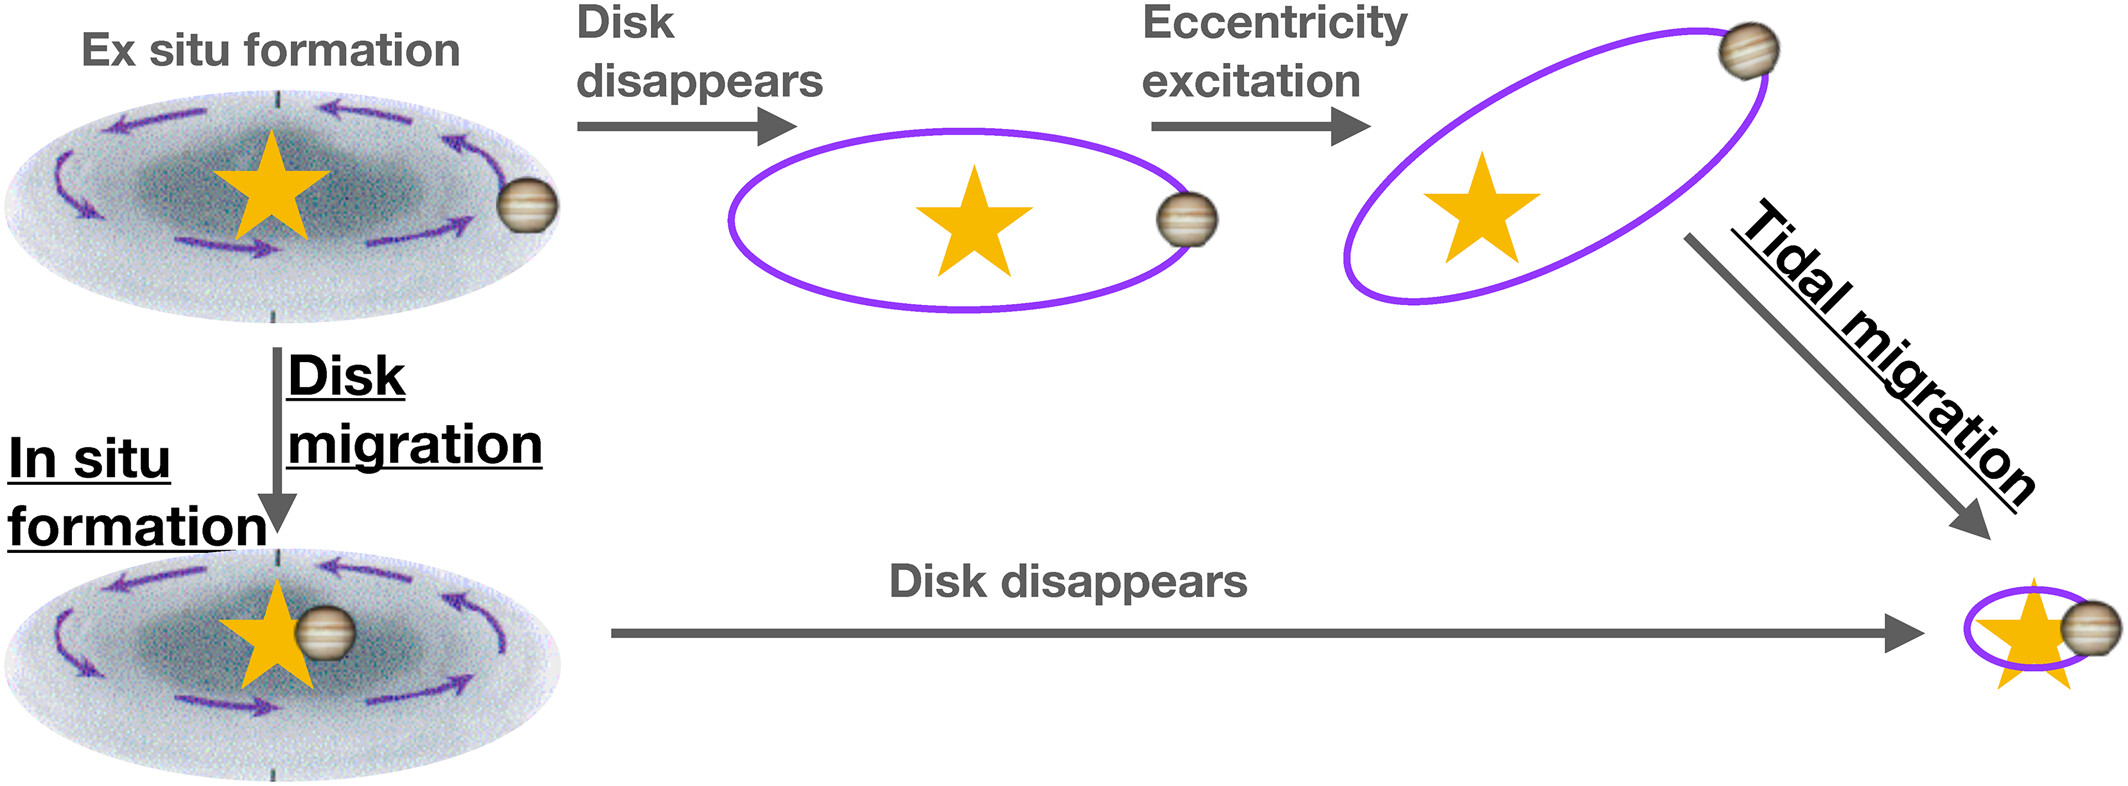
\includegraphics[width=\linewidth]{figs/hj_formation_theories.jpg}
    \caption{Pulled from \citet{fortney2021hotjupiters}, illustration of the leading formation theories of close-in gas giants: in-situ formation, disk migration, and high-eccentricity tidal migration.}
    \label{fig:formation-theories}
\end{figure}

In the early stages of a star's life, gas and small particles orbit around it, forming a protoplanetary disk—the birthplace of planets. \citet{fortney2021hotjupiters} and \citet{dawson2018origins} propose three main mechanisms for giant planet formation within this disk: in-situ formation, where the planet forms at its present-day orbital period; disk migration, where interactions with surrounding material drive the planet’s orbit inward; and high-eccentricity migration, where gravitational interactions with another body excite the planet’s orbit, followed by recircularization, which results in its current orbital period.

In situ formation, where a planet forms at its current orbital period close to its host star, can occur through core accretion, in which a planetary core accumulates a gaseous envelope to form a gas giant, or gravitational instability, where self-gravitating clumps form directly within the protoplanetary disk \citep{helled2013giant}. However, both mechanisms are highly contested.

\citet{dawson2018origins} argue that while core accretion can amass enough gas to form a gas giant, the required initial core—about 10 Earth masses—is difficult to form within the short orbital periods of hot Jupiters and the limited lifespan of the protoplanetary disk (which supplies the gas for accretion). Similarly, \citet{fortney2021hotjupiters} highlight several challenges: insufficient material within the disk to build a massive core, the protoplanetary disk preventing smaller cores from merging, and stalled pebble accretion before reaching the necessary 10 Earth masses. These issues align with the theories presented by \citet{dawson2018origins}, leading to the overall conclusion that core accretion may not be feasible for hot Jupiter formation.

Theories of gravitational instability face similar issues. \citet{dawson2018origins} note that the high temperatures and short orbital periods of hot Jupiter regions prevent gas from collapsing under its own gravity, making this mechanism unlikely as well. As a result, neither theory of close-in formation is widely accepted.

Outside the orbital period range of hot Jupiters, both core accretion and gravitational instability become much more viable mechanisms for planet formation. Hot Jupiters can initially form farther from their present-day orbits and migrate inward due to torques from the protoplanetary disk. However, \citet{fortney2021hotjupiters} and \citet{dawson2018origins} emphasize that migration is highly sensitive to disk conditions. If other forces—such as angular momentum transfer from the star or stalling due to a magnetocavity in the protoplanetary disk—fail to halt migration, the planet may continue inward past the hot Jupiter zone, ultimately being engulfed by its host star.

Another proposed mechanism for inward migration within the protoplanetary disk is high-eccentricity tidal migration. This process occurs when another object in the disk—most likely another forming planet—perturbs the gas giant’s orbit, extracting angular momentum and increasing its eccentricity. As the planet settles into an elongated orbit, gravitational interactions with its host star eventually cause the orbit to recircularize, with the final semimajor axis given by

\begin{equation}
    a_{\text{final}} = a(1 - e^2)
    \label{eq:final_semimajor_axis}
\end{equation}

where $a_{\text{final}}$ is the planet’s final semimajor axis after recircularization, $a$ is the original semimajor axis of its elongated orbit, and $e$ is the orbital eccentricity \citep{dawson2018origins}.

This theory is strongly supported by observations of warm Jupiters—planets thought to be precursors to hot Jupiters, with orbital periods between 10 and 200 days. Many warm Jupiters have eccentric orbits, and when recircularized, their final semimajor axes correspond to orbital periods of less than 10 days, aligning with the expected outcome of high-eccentricity tidal migration.

Consider the case of a recently studied exoplanet, TIC 393818343 b. In a recent paper, \citet{sgro2024confirmation} used ground-based observations to confirm that the planet has a non-zero eccentricity and an orbital period of approximately 16 days. If its orbit were to eventually recircularize, applying the observed orbital parameters to equation \ref{eq:final_semimajor_axis} yields a final orbital period of about 8 days—placing it well within the hot Jupiter region.

Across all formation theories, it is possible that planets initially form beyond their current orbital periods, migrate inward through disk migration or high-eccentricity tidal migration, and then continue migrating even after the protoplanetary disk dissipates due to gravitational interactions with their host stars. This continued inward migration may explain the existence of ultra-hot Jupiters (UHJs)—a subset of gas giants with orbital periods of less than three days.

UHJs provide a unique window into the final stages of hot Jupiter orbital evolution. Due to their large masses and extreme proximity to their host stars, UHJs exert strong gravitational forces, inducing significant tidal bulges on their stars—features that, in some cases, can even be directly observed \citep{barros2022detection}. The tidal bulge and the exoplanet tend to move toward synchronization; however, if the planet orbits faster than the tidal bulge rotates—causing the bulge to lag behind—angular momentum is transferred from the planet’s orbit to the star \citep{ogilvie2014tidal}. This loss of angular momentum causes the planet's orbit to shrink and the planet gradually spirals into its host star, a process known as orbital decay due to tidal interactions, or tidal decay. If no other mechanism intervenes to stall this process, these planets are expected to eventually undergo mass loss and ultimately be destroyed by their stars. A more in-depth review of this process is presented in Section \ref{sec:tidaldissipation}.

\textbf{TODO:} Should I add in information about merger outcomes using this paper: \citet{metzger2012optical}. This would cover stable/unstable mass loss, roche lobe overflow
- fills roche lobe below the stellar surface -> direct impact merger event
    - this has been potentially observed by \citep{de2023infrared}
- fills roche lobe above the stellar surface -> 
    - disrupted into an accretion disk around star called a tidal disruption merger event
    - gradually transfers mass over a long time scale called stable mass transfer

The theory of orbital evolution leading to planetary destruction is supported by observations showing that most UHJs are found around younger stars compared to the broader population of planet-hosting stars \citep{hamer2019hot}, suggesting that hot Jupiters do not "stick around" for long. However, only one confirmed hot Jupiter, WASP-12 b, has been observed undergoing tidal decay \citep{yee2019orbit}. This raises important questions: Are UHJs actively spiraling into their stars? If so, on what timescale does this occur? Or do other mechanisms stall or delay their destruction? Understanding the orbital evolution of UHJs is key to answering these questions.

\begin{figure}[htbp]
    \centering
    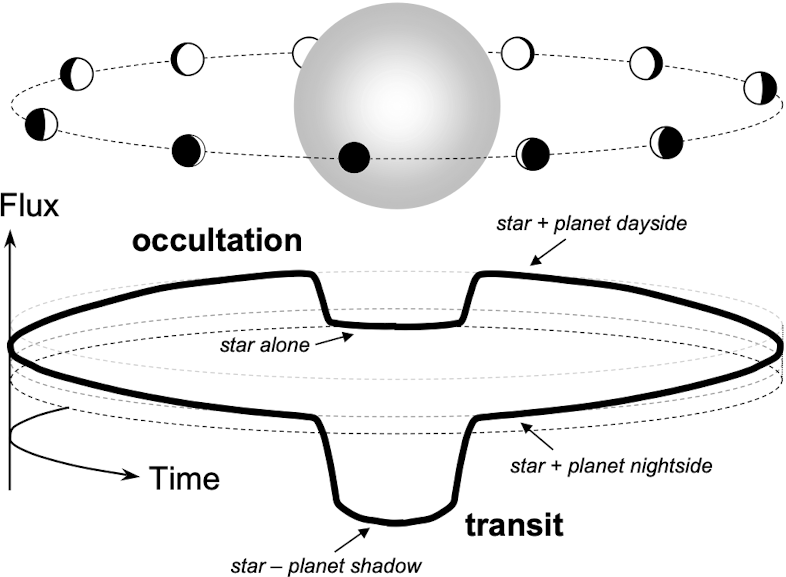
\includegraphics[width=0.7\linewidth]{figs/winn_fig1.png}
    \caption{Figure 1 from \citet{winn2010transits} illustrates an exoplanet transit and occultation edge-on. During a transit, the planet passes in front of its host star, blocking starlight and causing a characteristic dip in flux over time. During an occultation, the planet moves behind the star, obscuring its reflected light and producing a smaller flux dip.}
    \label{fig:winnfig1}
\end{figure}

There are multiple ways to observe the shrinking orbital periods indicative of tidally decaying UHJs. The unique size and proximity of UHJs makes a particular method of observation easy—transit observations. A transit occurs when an exoplanet passes in front of its star from our point of view, casting a shadow and blocking some light coming from the star. If we collect the amount of light (also called flux) coming from the star over time into a graph called a light curve, we will see a characteristic dip in the amount of light coming from the star as the planet passes over and casts its shadow, as seen in Figure \ref{fig:winnfig1} \citep{winn2010transits}. There are a few reasons why UHJs are ideal for these types of observations. First, these gas giants have large radii, which tend to be even more inflated as they move closer to their stars due to internal heating caused by tidal interactions with their host stars \citep{ogilvie2014tidal}. Their large radii cast a larger shadow on their host star during transits, which appear as more distinct dips in their light curves, making the transit both easier to detect and less erroneous. UHJs also have short orbital periods, meaning they orbit extremely quickly around their host stars and therefore have a large amount of transits to observe in a small time frame. For example, if a star is available to observe during a period of one month and the exoplanet's orbital period is about 3 days, you could potentially observe 10 transits in just one month. 

UHJ's large radii and short orbital periods also provide the opportunity to observe an occultation, which is when the planet moves around its star revealing its dayside, reflecting light towards us and increasing the overall amount of light coming from the system, and then moves behind its star, blocking out the light reflected from the planet and resulting in another characteristic, albeit smaller, dip in the light curve. We are lucky to be able to observe occultations for a handful of these systems, as most exoplanets are too small to be able to get any signal from their occultations in light curves. Occultations can be useful to track the overall motion and possible shape of the orbit. 

\begin{figure}[htbp]
    \centering
    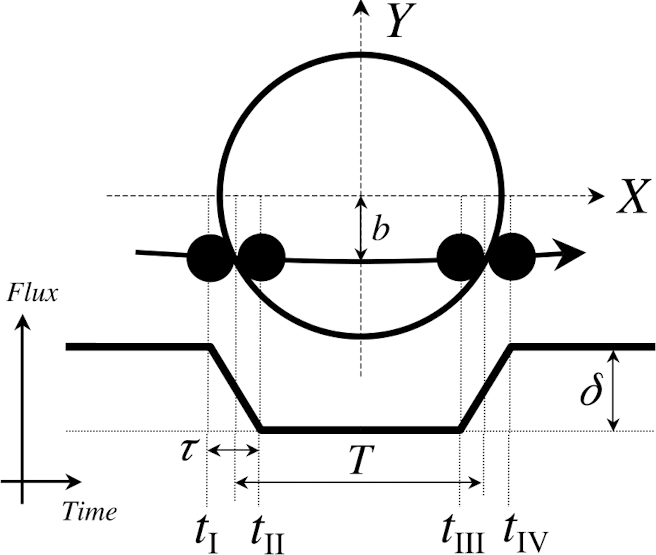
\includegraphics[width=0.6\linewidth]{figs/winn_fig2.png}
    \caption{Figure 2 from \citet{winn2010transits} illustrates the four key contact points during an exoplanet transit. First contact ($t_I$) marks the start of the transit when the planetary and stellar disks first touch. Second contact ($t_{II}$) occurs when the planet is fully within the stellar disk, defining the ingress duration ($\tau_\text{ing} = t_{II} - t_I$). Third contact ($t_{III}$) happens when the planet has moved across the stellar disk and begins to exit, and fourth contact ($t_{IV}$) marks the end when the disks last touch, defining the egress duration ($\tau_\text{egr} = t_{IV} - t_{III}$). The total duration ($T_\text{tot} = t_{IV} - t_{I}$) spans the entire transit, while the full transit duration ($T_\text{full} = t_{III} - t_{II}$) covers the time the planet is fully within the stellar disk.}
    \label{fig:winnfig2}
\end{figure}

UHJs have easily collectible light curves, but how do we process the data from these light curves? Let's call the time that the planet is in the very middle of its transit the midtransit time, which is calculated as half of the time it takes from contact two to contact three, $\frac{T_{\text{tot}}}{2}$, shown in Figure \ref{fig:winnfig2}. The time it takes from one consecutive midtransit time to the next is the amount of time it takes for the planet to complete one orbit around its star, which we call the orbital period. As we collect light curves, and therefore, midtransit times, of UHJ transits, we can observe the behavior of the orbital period over time. If the orbital period is consistent, then we may conclude that the UHJ's orbit is stable and unchanging. However, if we observe a change or even a decrease in the orbital period, we may conclude that the orbit is decaying, possibly due to tidal interactions with its host star, that will lead to its eventual inspiral. 

\begin{figure}[htbp]
    \centering
    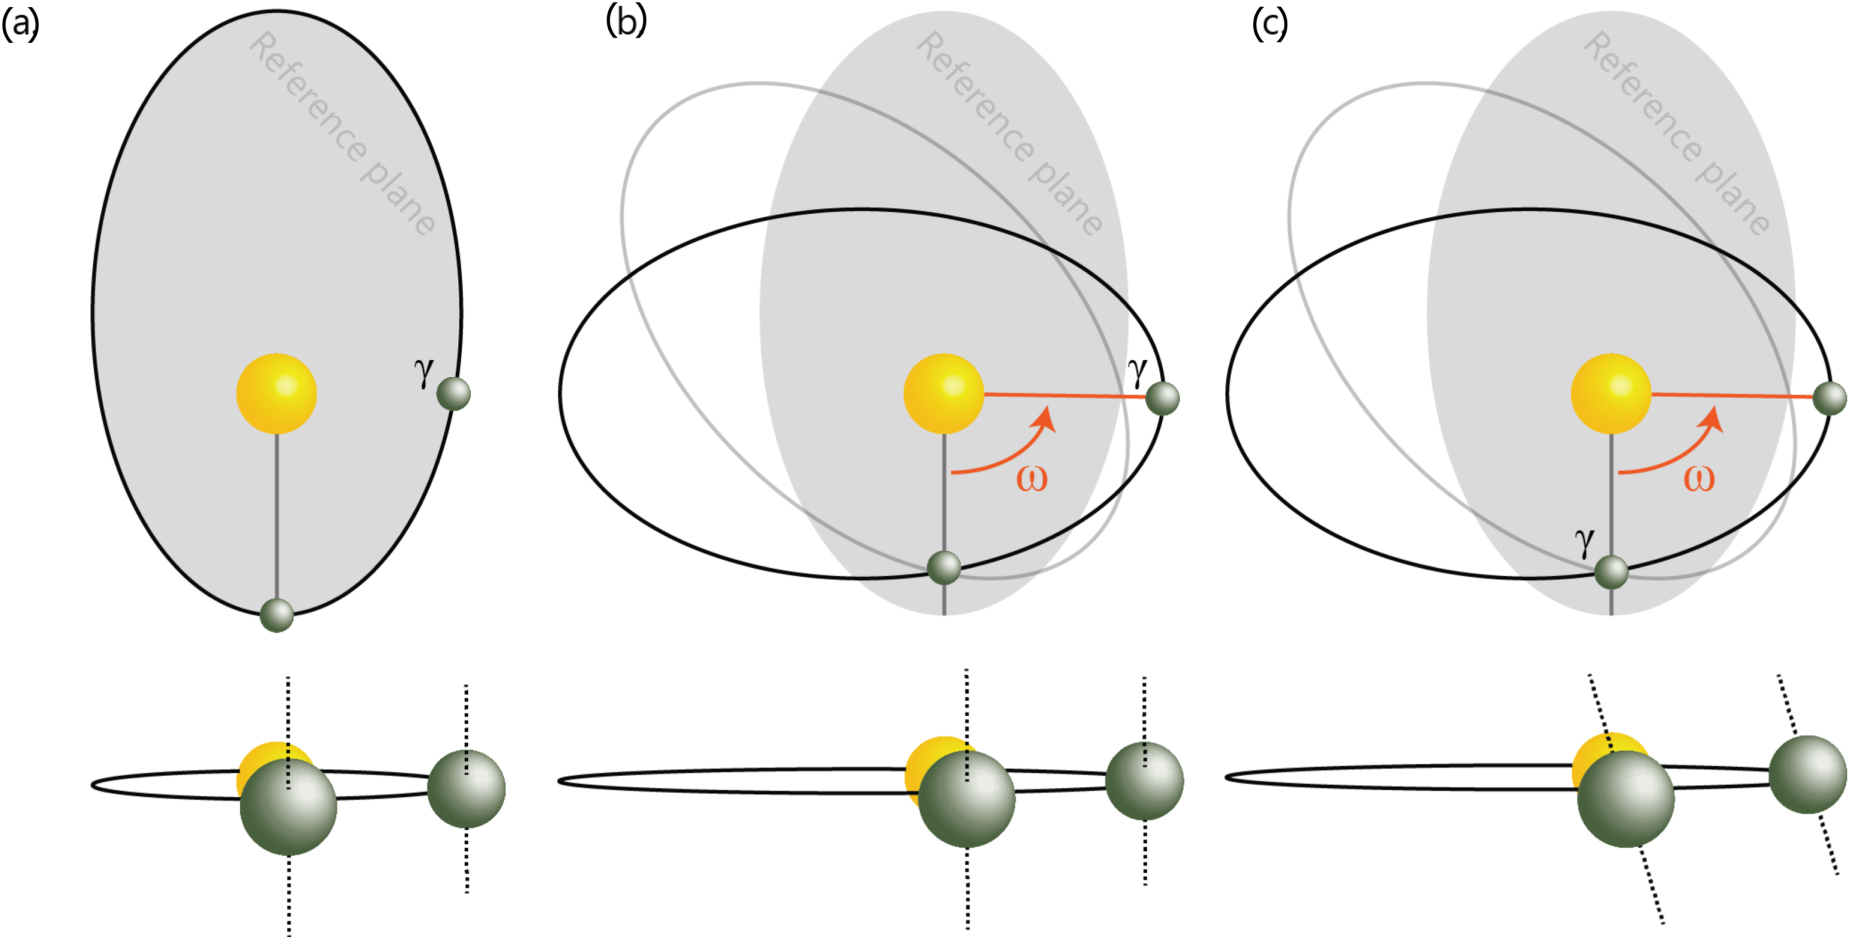
\includegraphics[width=0.8\linewidth]{figs/precession.jpg}
    \caption{Adapted from \citet{vervoort2022system}, this illustration depicts apsidal precession. The left panel shows an exoplanet initially orbiting within a fixed reference plane. Over time (right panel), the planet’s orbital ellipse precesses, gradually rotating within its plane. When observed edge-on, this precession causes variations in transit mid-times, making it appear as though the orbital period is changing. Without careful analysis, such shifts could be misinterpreted as evidence of tidal decay.}
    \label{fig:precession}
\end{figure}

Changes in the orbital period may not always indicate tidal decay. The orbital period may also change due to apsidal precession, which occurs when a planet's orbit rotates within its orbital plane, illustrated in Figure \ref{fig:precession}. This evolution can cause the time between transits to vary sinusoidally. However, precession also shifts the timing of occultations by an amount of time equivalent to but opposite in sign from the shift in transit timing. In contrast, if a planet's transit timing changes due to orbital decay, then the times between occultations decrease along with the times between transits.

Due to their large radii and short orbital periods, UHJs are prime targets for transit and occultation observations, enabling astronomers to track small orbital timing variations. These variations reveal key orbital properties and the planet’s interaction with its host star over time. While only one exoplanet is confirmed to undergo tidal decay, ongoing observations—by both professional and amateur astronomers—are expanding databases. As observations grow, orbital changes become clearer, improving our understanding of extrasolar systems. Ultimately, these efforts will help answer how UHJs formed and what their eventual fates are.

\clearpage




\subsection{Mechanisms of Tidal Dissipation in Stars and Giant Planets}\label{sec:tidaldissipation}

\subsubsection{Overview of Tidal Dissipation}
Summarize the mechanisms of tidal dissipation in stars and giant planets, as discussed by Ogilvie (2014).



\subsubsection{Application to UHJ Systems}
Discuss how these mechanisms apply to UHJs, considering their close proximity to host stars and the resulting strong tidal forces.

\begin{figure}[htbp]
    \centering
    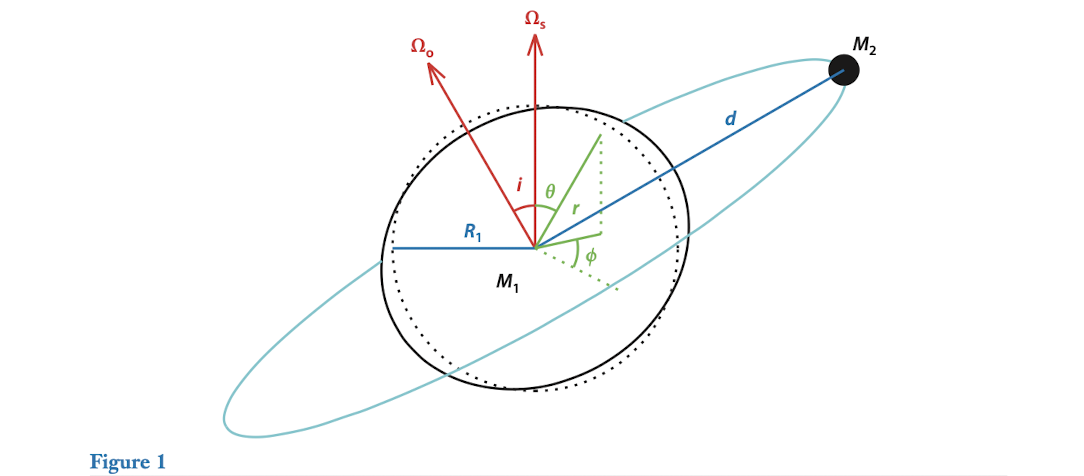
\includegraphics[width=\linewidth]{figs/ogilvie_fig1.png}
    \caption{Figure 1 from \citet{ogilvie2014tidal} illustrates the geometry of tidal interactions between two bodies. Shown here are the spherical polar coordinates ($\theta$, r, and $\phi$, in green) of the orbital planes, centered on body 1 with mean radius $R_1$ and mass $M_1$, and body 2 with mass $M_2$, with orbital separation $d$. $\Omega_s$ is the spin angular velocity vector and $\Omega_o$ is the orbital angular velocity vector, shown in red. The ellipsoidal bulge raised on body 1 by body 2 is shown by the solid black line, while the unaltered, spherical shape of body 1 is shown by the dotted black line.}
    \label{fig:ogilvie-fig1}
\end{figure}

In physics, many systems can be characterized by their monopole and quadrupole moments. The monopole moment is the simplest case, where a body is treated as a point mass with all its mass concentrated at a single point. The quadrupole moment accounts for non-uniform mass distributions, describing bodies that deviate from a perfect sphere, such as UHJs with tidal bulges.

Tidal interactions typically involve the monopole moment of one body and the quadrupole moment of the other \citep{ogilvie2014tidal}. As illustrated in Figure \ref{fig:ogilvie-fig1}, we can model the interaction between a UHJ and its host star by treating the star as a monopole (a point mass) and the planet as a quadrupole, since the star’s gravity raises a tidal bulge on the planet. While simplified in the figure, this bulge is not perfectly aligned with the axis connecting the two bodies; instead, it is slightly offset. This misalignment induces tidal forces that transfer angular momentum and dissipate energy. Over time, these forces drive the system toward tidal locking, where the planet’s rotation period matches its orbital period, causing the same hemisphere to always face its host star.

Over time, tidal forces drive a system toward tidal equilibrium, in which both bodies achieve aligned, synchronous rotation and a circular orbit. However, in systems with large mass differences, such as UHJ systems, this equilibrium may not be possible because the total angular momentum of the system is insufficient.

The total angular momentum of a system is the sum of orbital angular momentum ($L_o$)–the angular momentum associated with the planet's orbit around its host star—and the spin angular momentum ($L_s$)–the angular momentum from the planet’s rotation about its own axis.
For tidal equilibrium to be reached, the total angular momentum ($L = L_o + L_s$) must exceed a critical threshold ($L_c$). If $L < L_c$, the system continues evolving instead of settling into a stable state.

In extreme mass ratio systems, the smaller body contributes very little spin angular momentum because its moment of inertia is small. As a result, the total angular momentum is much lower than in systems with two similar-mass bodies (such as binary stars), where both contribute significant spin angular momentum. If the system cannot reach equilibrium, tidal interactions continue to transfer angular momentum between the planet’s orbit and the star’s spin. Over time, this exchange causes the planet’s orbit to decay, ultimately leading to orbital inspiral and destruction as the planet is pulled into its host star.

% In circular orbits, rotation speed matches orbit and the spin axis aligns to straight-up direction relative to the orbital plane. However, in eccentric orbits, the tidal forces are strongest at the pericenter, so the spin usually synchs at the fastest part of the orbit, entering a state of psuedo-synchronization. If we consider the warm to hot jupiter theory represented in \citep{fortney2021hotjupiters} and \citep{dawson2018origins}, if we start with an eccentric orbit, then the planet will enter pseudo-synchronization 

\begin{figure}[htbp]
    \centering
    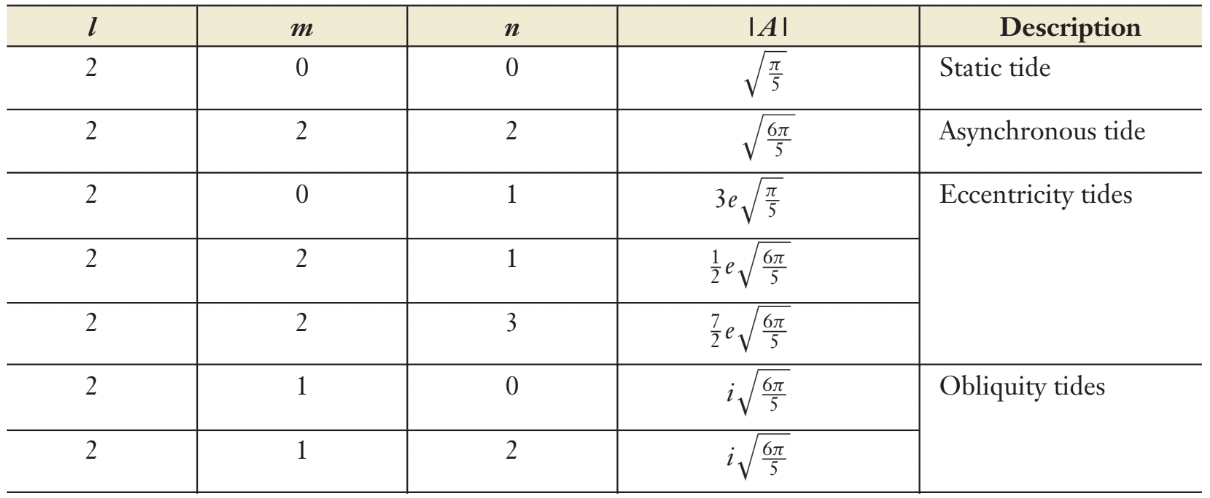
\includegraphics[width=\linewidth]{figs/ogilvie_tbl1.png}
    \caption{Table 1 from \citep{ogilvie2014tidal} shows the quadrupolar components of the tidal potential. }
    \label{fig:ogilvie-tbl1}
\end{figure}

\begin{figure}[htbp]
    \centering
    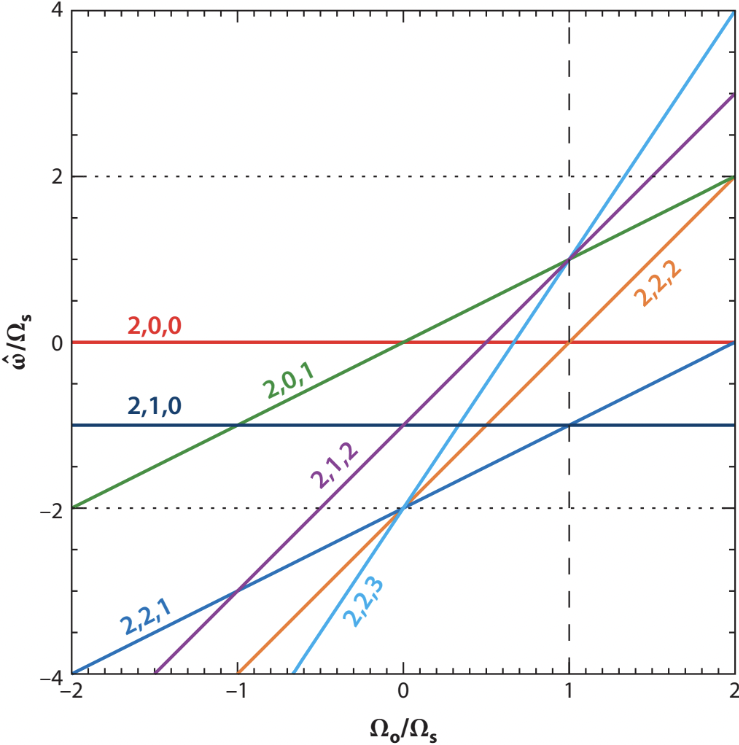
\includegraphics[width=0.8\linewidth]{figs/ogilvie_fig2.png}
    \caption{The vertical axis describes the tidal frequency in the fluid frame, which is the angular frequency measured in frame of reference rotating with the body ($\hat{\omega}$), divided by the body's spin frequency ($\Omega_s$). This tells us how the tidal forces compare to the body's own revolution about its axis. The horizontal axis is the orbital frequency ($\Omega_o$), which is the rate that body 1 rotates around body 2, divided by the spin frequency ($\Omega_s$), which is the rate that body 1 spins about its axis. This tells us how fast the body is orbiting compared to its spin. The body reaches a synchronous state at $\frac{\Omega_o}{\Omega_s} = 1$, which is indicated by the dashed vertical line. 
    Each colored line represents a different set of quadrupolar components of the tidal potential found in Table \ref{fig:ogilvie-tbl1}, labeled by $l, m, n$. Each line has slope $n$, which is the temporal harmonic index, or the time-dependent components of the quadrupolar components, and y-intercept $-m$, which is the order of spherical harmonic, which determines the longitudinal structure of the tide.
    Dotted lines indicate the frequency at which inertial waves can be excited inside the rotating body.}
    \label{fig:ogilvie-fig2}
\end{figure}

The tidal potential, which describes the gravitational influence of one body on another, is commonly expressed using spherical harmonics. Spherical harmonics provide a mathematical framework to expand the tidal potential into multipole moments, solving partial differential equations to describe different spatial variations. The most significant moments are the monopole moment ($l = 0$), where the body is treated as a point mass, and the quadrupole moment ($l=2$), which accounts for the body's deviation from a perfect sphere due to tidal distortions.

% EXPLAINING TABLE 1

Table \ref{fig:ogilvie-tbl1} lists the quadrupolar components of different tidal contributions. All tides in the table have $l=2$, describing the behavior of a tidal bulge raised on the body.

The order of the spherical harmonic, $m$, represents the longitudinal structure of the tidal bulge. When $m=0$, the tides are axisymmetric, meaning the bulge is uniformly distributed around the entire body. When $m=1$ or $m=2$, the tides are non-axisymmetric, meaning the bulge varies with longitude.

The temporal harmonic index, $n$, represents the time-dependent components of the tidal potential. If $n=0$, the tide is static, leading to a constant deformation. If $n>0$, the tide oscillates periodically due to orbital motion.

The tidal amplitude, $|A|$, describes the relative strength of each tidal component. 

A static tide, corresponding to $n=0$ and $m=0$, represents a permanent, axisymmetric tidal bulge raised on the body. An asynchronous tide, corresponding to $l=m=n=2$, occurs when the body's spin is not synchronized with its orbit, leading to the misalignment between the tidal bulge and the orbital motion. An eccentricity tide arises from an elliptical orbit, with its amplitude $|A|$ proportional to the orbital eccentricity $e$, leading to periodic variations in tidal forces due to varying speeds as the body moves through its orbit. An obliquity tide is driven by a misalignment between the body's spin axis and its orbital plane, with its amplitude $|A|$ proportional to the obliquity $i$ (the measure of the tilt relative to the orbital plane), introducing additional tidal components that depend on the body's tilt.

Figure \ref{fig:ogilvie-fig2} plots the seven sets of quadrupolar components from Table \ref{fig:ogilvie-tbl1}. 

% INTERPRETING FIG \ref{fig:ogilvie-fig2}

The Coriolis force (EXPLAIN) can give rise to inertial waves in a rotating body. If a full sphere is fully convective, such as a star, then inertial waves can propagate. Tidal response (explain) of inertial waves increase with the spin frequency of the rotating body, meaning bodies that spin faster have higher tidal responses and higher rates of tidal dissipation. Larger cores or greater density contrasts between layers lead to stronger tidal responses in inertial waves. (idk how this exactly ties into UHJS)

Based on the formation theories, the inertial waves may differ greatly. If it is the in-situ formation, there is a theorized minimum 10 earth mass core, which is fairly large and therefore has higher tidal dissipation rates. 

These are important because tidal dissipation rate depends heavily on the frequency of these waves. When tidal component frequency (y-axis) falls within the range of inertial waves (dotted horizontal lines), the mode can interact with fluid motions and enhance tidal dissipation. The presence of strong tidal interactions when internal waves are excited may explain the high tidal dissipation rates we see in UHJ systems.

Dissipation rates within the planet can explain tidal circularization, while dissipation rates within the star can explain transfer of angular momentum and orbital decay.

When the orbital and spin angular frequencies of a body are equal to one another, they reach a synchronous state in which the body is orbiting at the same rate that it is spinning on its axis. This state is shown by the dashed vertical line in Figure \ref{fig:ogilvie-fig2}. This can influence the long-term tidal evolution HOW??

\begin{figure}[htbp]
    \centering
    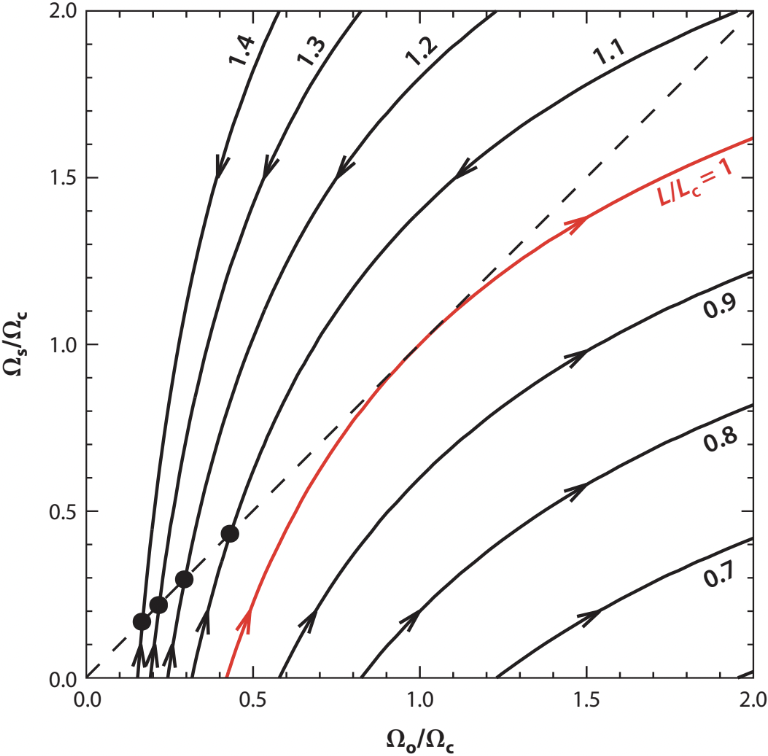
\includegraphics[width=0.8\linewidth]{figs/ogilvie_fig10.png}
    \caption{The evolutionary paths of a planet interacting with its host star (assuming a circularized orbit with $e=0$). The vertical axis shows the stellar spin angular frequency (in units of the critical angular velocity, $\Omega_c$, which is associated with the critical angular momentum, $L_c$, which is the angular momentum needed to reach tidal equilibrium). The horizontal axis shows the stellar orbital angular velocity (also in units of critical angular velocity $\Omega_c$). The solid lines are contours of the total angular momentum $L$. The dashed line represents the stellar synchronized state, when the spin and orbital angular frequencies are equal. Black points are moments of tidal equilibrium, when $L \geq L_c$. If tidal equilibrium is not reached, when $L < L_c$, then the planet heads towards destruction.}
    \label{fig:ogilvie-fig10}
\end{figure}

If the total angular momentum, $L$, is less than the critical value $L_c$, then the orbital angular momentum of the planet is turned into stellar spin angular momentum, leading to a decaying orbit and stellar spin-up. 

When looking at binary star recircularization, we find a tidal dissipation rate $Q^{'}_{*}$ of $10^6$. However, if we assume this rate for UHJ systems, we get unrealisticly short orbital decay timescales. As seen in JACKSON PAPER, ADAMS PAPER (maybe use adams table 8), if we assume a constant value of $Q^{'}_{*}$, we get the following theoretical dP/dE, which differs from the observed dP/dE. This shows that we cannot assume this value, and that it is instead dependent on things such as stellar structure blah blah. 

The galactic engulfment rate scales with the tidal dissipation rate. So, if we can constrain the tidal dissipation rate, then we can constrain the galactic engulfment rate and have a rough estimate of how many merger events occur in our galaxy each year. BUT WHAT IF THE TIDAL DISSIPATION RATE IS NOT THE SAME FOR EACH SYSTEM??? 

\begin{figure}[htbp]
    \centering
    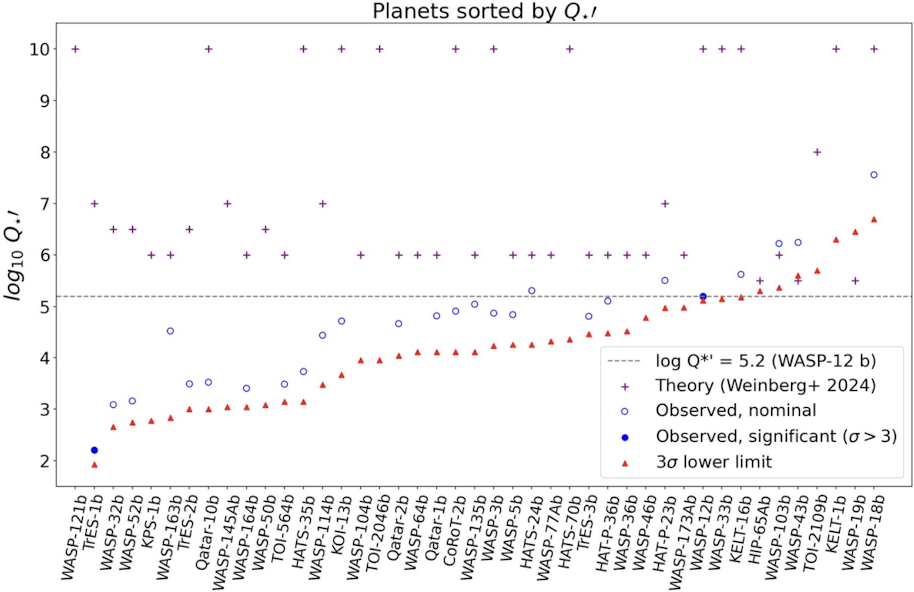
\includegraphics[width=\linewidth]{figs/adams_fig11.png}
    \caption{Caption}
    \label{fig:adams-fig11}
\end{figure}


\clearpage

\subsection{Detection and Analysis of Transits and Occultations}

\subsubsection{Photometric Techniques}
Review the methods for detecting transits and occultations, as outlined by Winn (2010).

\subsubsection{Relevance to Orbital Decay Studies}
Explain how precise measurements of transit timings can indicate changes in orbital periods, signaling potential tidal decay.





\subsection{Analytical Approaches to Transit Light-Curve Observables}

\subsubsection{Analytical Models}
Discuss the analytical approximations for transit light-curve observables presented by Carter et al. (2008).

\subsubsection{Implications for Detecting Orbital Decay}
Examine how these models assist in accurately determining transit times and detecting minute changes indicative of orbital decay.





\subsection{Metrics for Optimizing Searches for Tidally Decaying Exoplanets}

% Describing delta BIC
For these planets, we are particularly interested in the decreasing orbital periods when searching for tidal decay. Increasing orbital periods, while interesting, do not indicate tidal decay and therefore are not of interest to us in this instance. 

When fitting a model, we determine the accuracy of the model fit to the actual data using the Bayesian Information Criterion (BIC) \citep{schwarz1978estimating}

\begin{equation}
    \text{BIC} = \chi^{2} + k\text{ln}N
\end{equation}

where $k$ is the number of fit parameters (two for a linear model, three for a quadratic model, and five for a precession model), $N$ is the number of data points or observations used to fit the model, and $\chi^{2}$ is the reduced chi-squared, which is the measurement of the goodness of fit, calculated by the sum of the residuals squared \citep{pearson1900criterion}:

\begin{equation}
    \chi^{2} = \sum \left( \frac{O_i - E_i}{\sigma_i} \right)^2
\end{equation}

where $O_i$ is the actual observed value, $E_i$ is the expected value calculated by the model, and $\sigma_i$ is the photometric uncertainty.

Smaller values of $\chi^2$ indicate smaller residuals, suggesting a better fit of the model to the data. However, models with more fit parameters can become biased, fitting the data too closely. For example, in Figure \ref{fig:reduced-chi-squared}, we compare three models fitted to synthetically generated data: a linear model with two parameters, a quadratic model with three parameters, and a sinusoidal model with five parameters. As the number of fit parameters increases, the $\chi^2$ value also rises, suggesting that more complex models may better explain the data pattern. However, when we account for the penalization of additional parameters using BIC, the value of BIC decreases, showing that more complex models do not necessarily provide a better description of the data. To minimize bias in more complex models, we use BIC, which adds a penalty based on the number of fit parameters $k$ to the reduced $\chi^2$ value.

\begin{figure}[htbp]
    \centering
    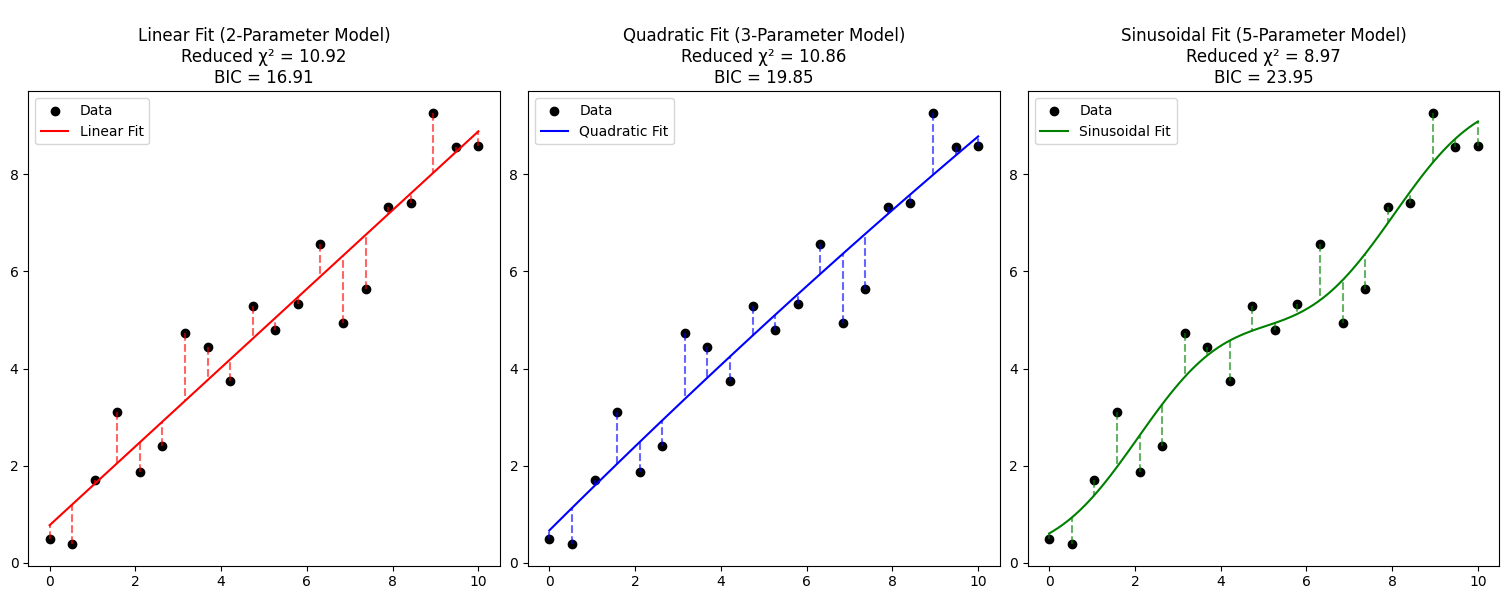
\includegraphics[width=\linewidth]{figs/reduced_chi_squared.png}
    \caption{Comparison of model fit analysis to synthetic data. Residuals, represented by the dashed lines, show the differences between the actual data (black circles) and the model fits (solid lines). The reduced $\chi^2$ and BIC values for each model are displayed above the corresponding plot.}
    \label{fig:reduced-chi-squared}
\end{figure}

In this case, positive values of $\Delta$ BIC, calculated with the equation:

\begin{equation}
    \Delta \text{BIC} = \text{BIC}_{\text{lin}} - \text{BIC}_{\text{quad}}
\end{equation}

indicate a statistical preference for a quadratic model over a linear model.

\begin{figure}[htbp]
    \centering
    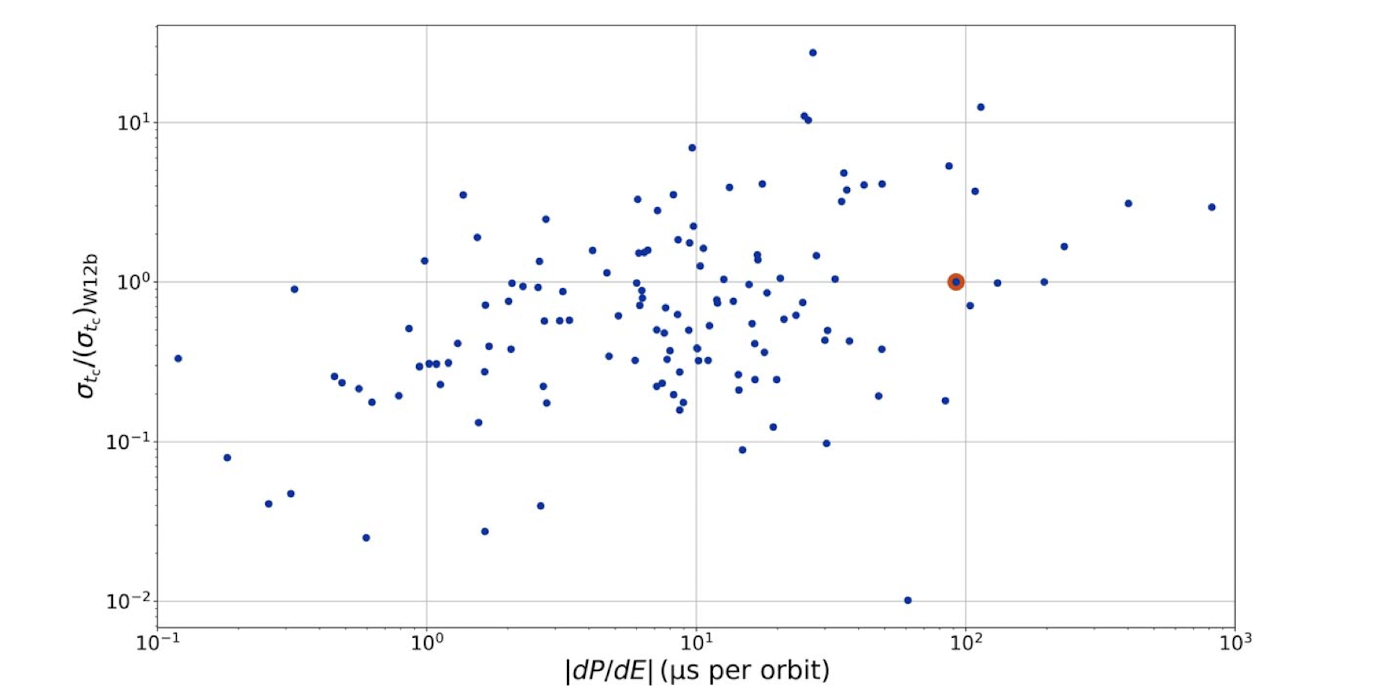
\includegraphics[width=\linewidth]{figs/jackson_fig1.png}
    \caption{The uncertainty on the mid-transit time for multiple extrasolar systems based on the simplified transit model from \citet{carter2008analytic}, normalized to WASP-12 b's mid-time uncertainty, versus the change in orbital period with respect to time.}
    \label{fig:jackson-fig1}
\end{figure}

The y-axis of Figure \ref{fig:jackson-fig1} in \citet{jackson2023metrics} shows the analytical uncertainties of transit mid-times using the equation:

\begin{equation}
    \sigma_{t_c} = \sqrt{\frac{\tau}{2\Gamma}} \left(\frac{\sigma}{\Delta}\right) = \sigma \Gamma^{-1/2}
    \times \left( \frac{R_\star}{a} \right)^{1/2} \left( \frac{P}{2\pi} \right)^{1/2} 
    \left( \frac{R_p}{R_\star} \right)^{-3/2} (1 - b^2)^{-1/4} 
    \times \begin{cases}
    1, & \text{transit} \\
    \left(\frac{I_p}{I_\star}\right)^{-1}, & \text{eclipse}.
    \end{cases}
    \label{eq:analytical_transit_uncertainties}
\end{equation}

where $\tau$ is the ingress/egress duration, $\Gamma$ is the sampling rate for the transit observations (assumed constant), $\sigma$ is the per-point photometric uncertainty, $\Delta$ is the transit or eclipse depth, $R_{*}$ is the stellar radius, $a$ is the orbital semimajor axis, $P$ is the orbital period, $R_{p}$ is the planetary radius, $b$ is the impact parameter, and $I_{p/*}$ is the planetary/stellar disk-integrated intensity. 

For comparison, uncertainties are normalized to the transit mid-time uncertainty of WASP-12 b, which is one of the only confirmed tidally decaying exoplanets. 

The x-axis of \ref{fig:jackson-fig1} shows the analytical orbital decay rate, defined as the change in orbital period over each consecutive orbit, also called an epoch, using the equation: 

\begin{equation}
    \frac{dP}{dE} = P \frac{dP}{dt} \approx - (26 \, \mu s \text{ per orbit})
    \times \left( \frac{M_p}{M_{\text{Jup}}} \right)
    \left( \frac{M_\star}{M_\odot} \right)^{-8/3}
    \left( \frac{R_\star}{R_\odot} \right)^{5}
    \times \left( \frac{P}{\text{day}} \right)^{-10/3}
    \left( \frac{Q_\star}{10^5} \right)^{-1},
    \label{eq:orbital_period_rate_of_change}
\end{equation}

where $\frac{dP}{dt}$ is the change in orbital period with respect to time, $M_p$ is the planetary mass in Jupiter masses ($M_{Jup}$=
1.89813 × 1027 kg), $M_*$ is the stellar mass in solar masses
($M_e$ = 1.989 × 1030 kg), $R_*$ is the stellar radius in solar radii ($R_e$ = 6.957 × 108 m), $P$ is the orbital period in days, and $Q_*$ is the star’s modified tidal dissipation parameter.

Figure \ref{fig:jackson-fig1} shows an upwards trend in this relationship, meaning as the rate of change of the planet's orbit increases, so does the uncertainty on its mid-transit time. So while systems with quickly changing orbital periods may be more interesting to focus on, the mid-time may be harder to predict, especially as time goes on. One thing to keep in mind with this figure is that the value of $\frac{dP}{dE}$ is based on equation \ref{eq:orbital_period_rate_of_change} with appropriate system parameters filled in, but assuming a WASP-12 b-like tidal dissipation parameter $Q_* = 2 \times 10^5$. However, in \citet{ogilvie2014tidal}, it is shown that the tidal dissipation parameter depends on stellar internal structure, which give rise to different spherical harmonics. Incorporating non-linear dissipation into theoretical models, \citet{weinberg2023orbital} found that the tidal dissipation parameter varies with stellar mass and age. Therefore, the value of $Q_*$ cannot be assumed to be constant for different extrasolar systems. For future work, an interpolable grid of $Q_*$ values would need to be generated based on stellar age and mass, and analytical approaches would need to incorporate a more refined estimate of the tidal dissipation parameter based on the stellar properties.

\begin{figure}[htbp]
    \centering
    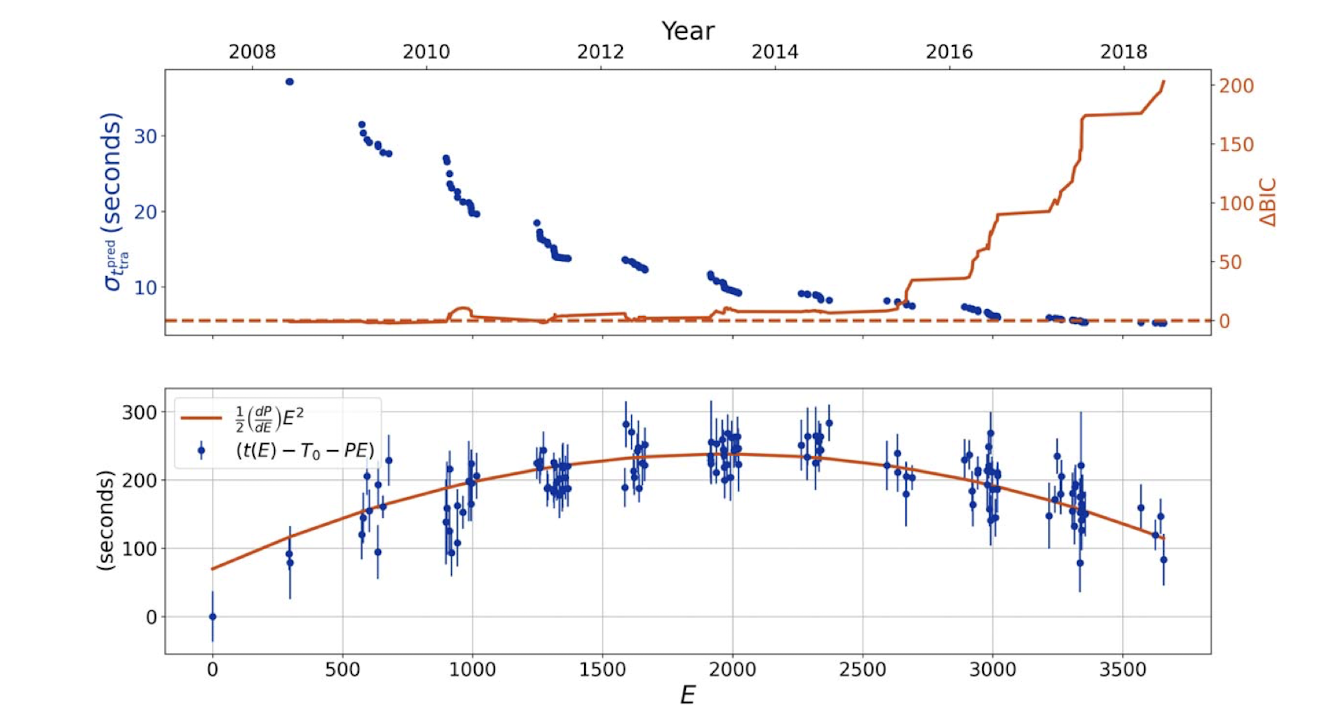
\includegraphics[width=\linewidth]{figs/jackson_fig2.png}
    \caption{(Top) The blue dots show the uncertainty on the predicted transit mid-time of WASP-12 b as observations increase. The orange line shows the value of $\Delta$BIC as observations increase. (Bottom) The blue dots show the observed transit mid-time with the linear ephemeris subtracted to show the trend in non-linear parameters (the orbital decay rate $\frac{dP}{dE}$). The orange line shows the quadratic ephemeris term $\frac{dP}{dE}$ = -86.7 $\mu$s orbit$^{-1}$, which is pulled from the orbital decay model in \citet{yee2019orbit}.}
    \label{fig:jackson_fig2}
\end{figure}

Figure 2 in \citet{jackson2023metrics} shows how different analytical approximations may change as observations increase using the example of WASP-12 b data pulled from \citet{yee2019orbit}. The left x-axis of the top figure shows the uncertainty of the predicted transit mid-time. The right x-axis of the top figure shows the value of $\Delta$BIC comparing a linear ephemeris to a quadratic ephemeris. The x-axis of the bottom figure shows the difference between the observed transit mid-time and the linear ephemeris fit in seconds. The y-axis for both figures uses epoch to denote consecutive orbits, with the associated year shown at the top to aid in understanding the passage of time between observations. 

As the system is observed over time, the quadratic term of the linear-subtracted mid-times becomes more apparent. However, in the initial observations, the trend may appear linear. 

As observations increase for the system, the uncertainty on the predicted transit mid-time decreases and the value of $\Delta$BIC increases, showing preference for a quadratic model. However, these observations are fairly consistent, with more observations added about every year. If enough time has passed between observations such that the uncertainty on the mid-time surpasses the transit duration, then it may be difficult to predict future transit mid-times. Such systems are ideal for follow-up observations. Figure \ref{fig:jackson_fig3} shows the amount of time needed between observations before the transit duration surpasses the predicted error on the mid-time given by the following equation:

\begin{equation}
    t_{wait} = \sqrt{\sigma^{2}_{t^{pred}_{tra}} - \sigma^{2}_{T_{0}}} \left(\frac{P}{\sigma_{P}} \right)
    \label{t_wait}
\end{equation}

versus the time since the last recorded observation as of April 5th, 2023. The labeled systems are close to or have surpassed their $t_{wait}$ value and need follow-up observations to confirm their predicted transit mid-time is what we expect (and if it is not what we expect, then this may indicate changes in the orbital period). 

\begin{figure}[htbp]
    \centering 
    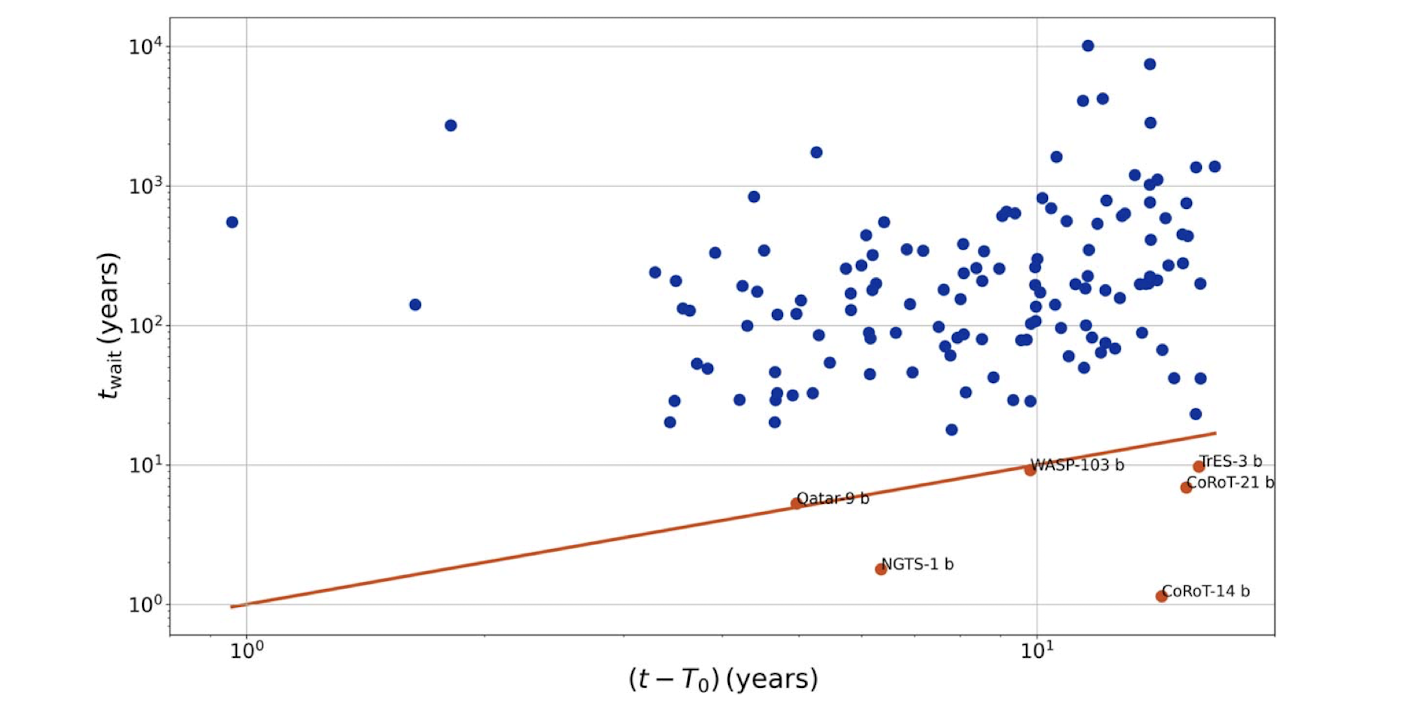
\includegraphics[width=\linewidth]{figs/jackson_fig3.png}
    \caption{Time needed to pass between observations for the uncertainty on the transit mid-time to surpass the transit duration ($t_{wait}$) versus the time that has passed since the first recorded transit ($T_0$) (generated April 5th, 2023). QUESTION: Is $T_0$ the first ever recorded transit or the time of conjunction or the last observed transit idk??????}
    \label{fig:jackson_fig3}
\end{figure}

% \subsubsection{Proposed Metrics}
% Summarize the metrics introduced by Jackson et al. (2023) for optimizing the search for tidally decaying exoplanets.

% \subsubsection{Application to UHJ Systems}
% Evaluate the effectiveness of these metrics when applied to UHJs, considering their unique characteristics.





\subsection{Observational Evidence and Challenges}

\begin{figure}[htbp]
    \centering
    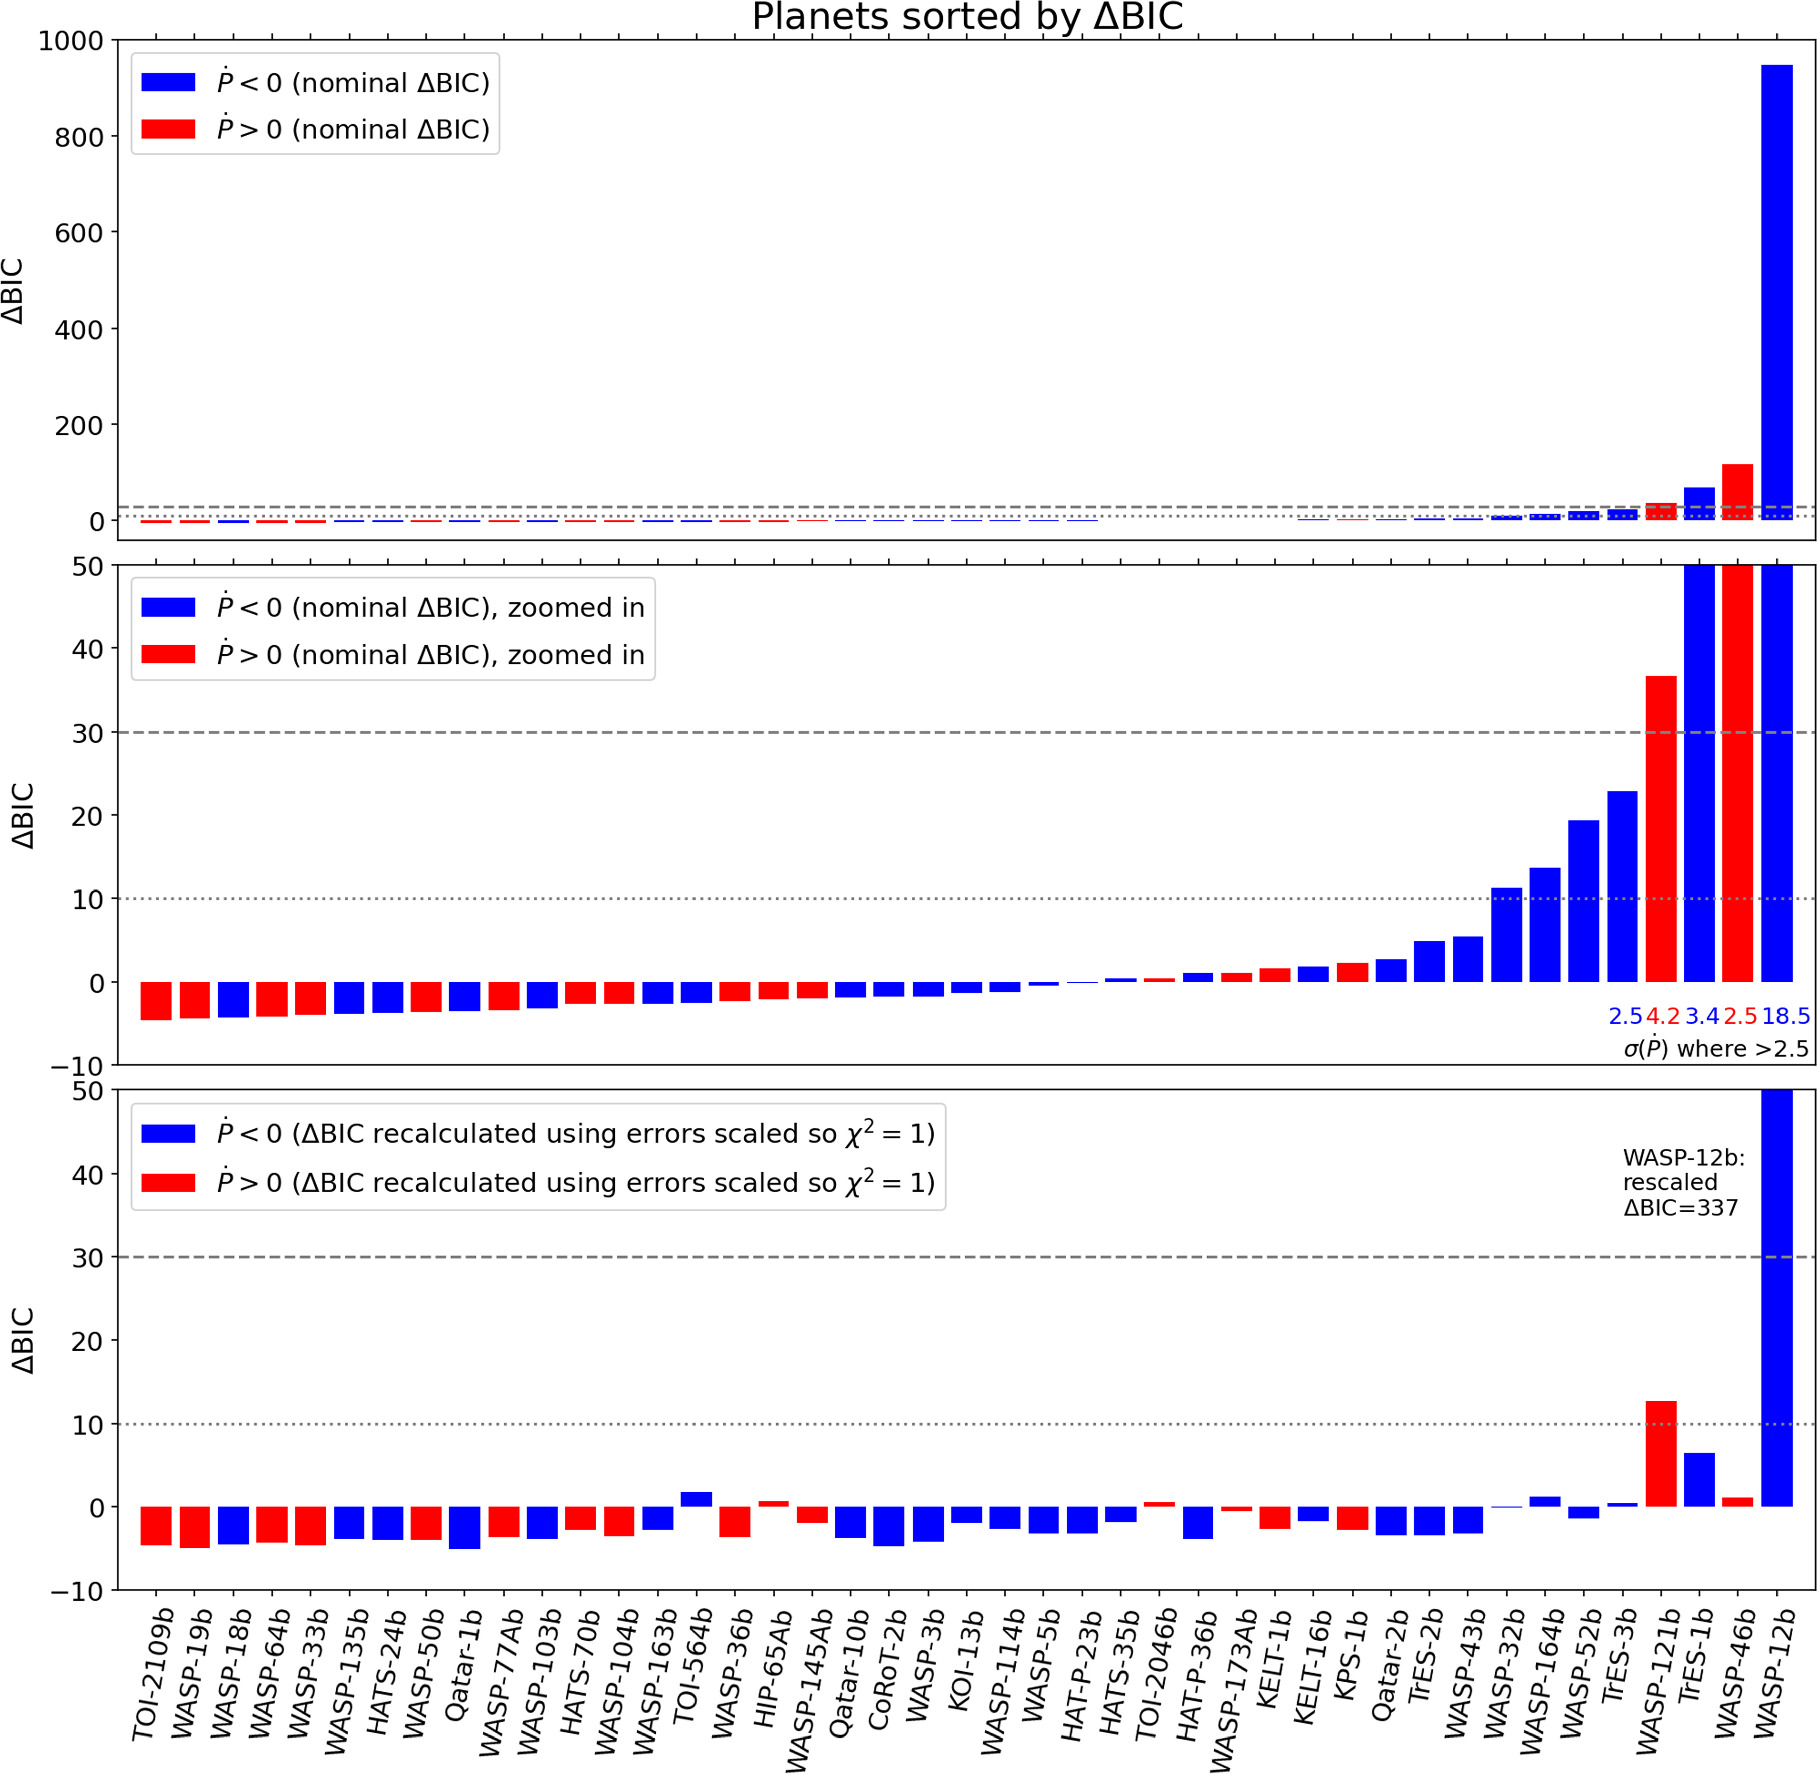
\includegraphics[width=0.9\linewidth]{figs/adams_fig2.jpg}
    \caption{$\Delta$BIC values for 43 exoplanets. In all panels, a positive $\Delta$BIC value favors a quadratic model over a linear model, indicating a change in the orbital period. Blue bars represent planets with a negative $\dot{P}$ (decreasing orbital period), while red bars indicate a positive $\dot{P}$ (increasing orbital period). Two reference lines are included: a dashed line at $\Delta$BIC = 30 and a dotted line at $\Delta$BIC = 10. 
    The top panel displays the full range of $\Delta$BIC values, with WASP-12 b standing out as a clear outlier. The middle panel zooms in to highlight the smaller $\Delta$BIC values, showing the five systems with the next highest $\Delta$BIC values after WASP-12 b. For these systems, uncertainties on their measured orbital period changes (P???) are plotted below the corresponding bars. The bottom panel presents the $\Delta$BIC values after applying a rescaling procedure to the data. Details of this rescaling process are discussed below.}
    \label{fig:adams-fig2}
\end{figure}

% Describing the rescaling process
In reported literature, uncertainties on mid-transit times in light curves can sometimes be unrealistically small. When fitting a model to transit data, each data point is weighted according to its photometric uncertainty, $\sigma$, with weights proportional to $\frac{1}{\sigma}$. If a data point has an exceptionally small uncertainty, it disproportionately influences the model fit, effectively "weighing down" the resulting model and skewing the fit toward that point.

To mitigate this issue, \citet{adams2024doomed} implemented a rescaling procedure. They first performed a linear fit using the original timing uncertainties and calculated the corresponding $\chi^2$ value. Then, they uniformly scaled all uncertainties by a factor such that the resulting $\chi^2$ value equaled 1. After rescaling, \citep{adams2024doomed} recomputed the $\Delta$BIC values for all systems, as shown in the bottom panel of \ref{fig:adams-fig2}. This adjustment significantly altered the $\Delta$BIC values, with only one system—excluding WASP-12 b—retaining a $\Delta$BIC greater than 10.

This change in $\Delta$BIC highlights the importance of data processing and accuracy. 

% TODO: Add a plot here to show how unrealistic transit midtime uncertainties can affect the resulting model fit.

\begin{figure}[htbp]
    \centering
    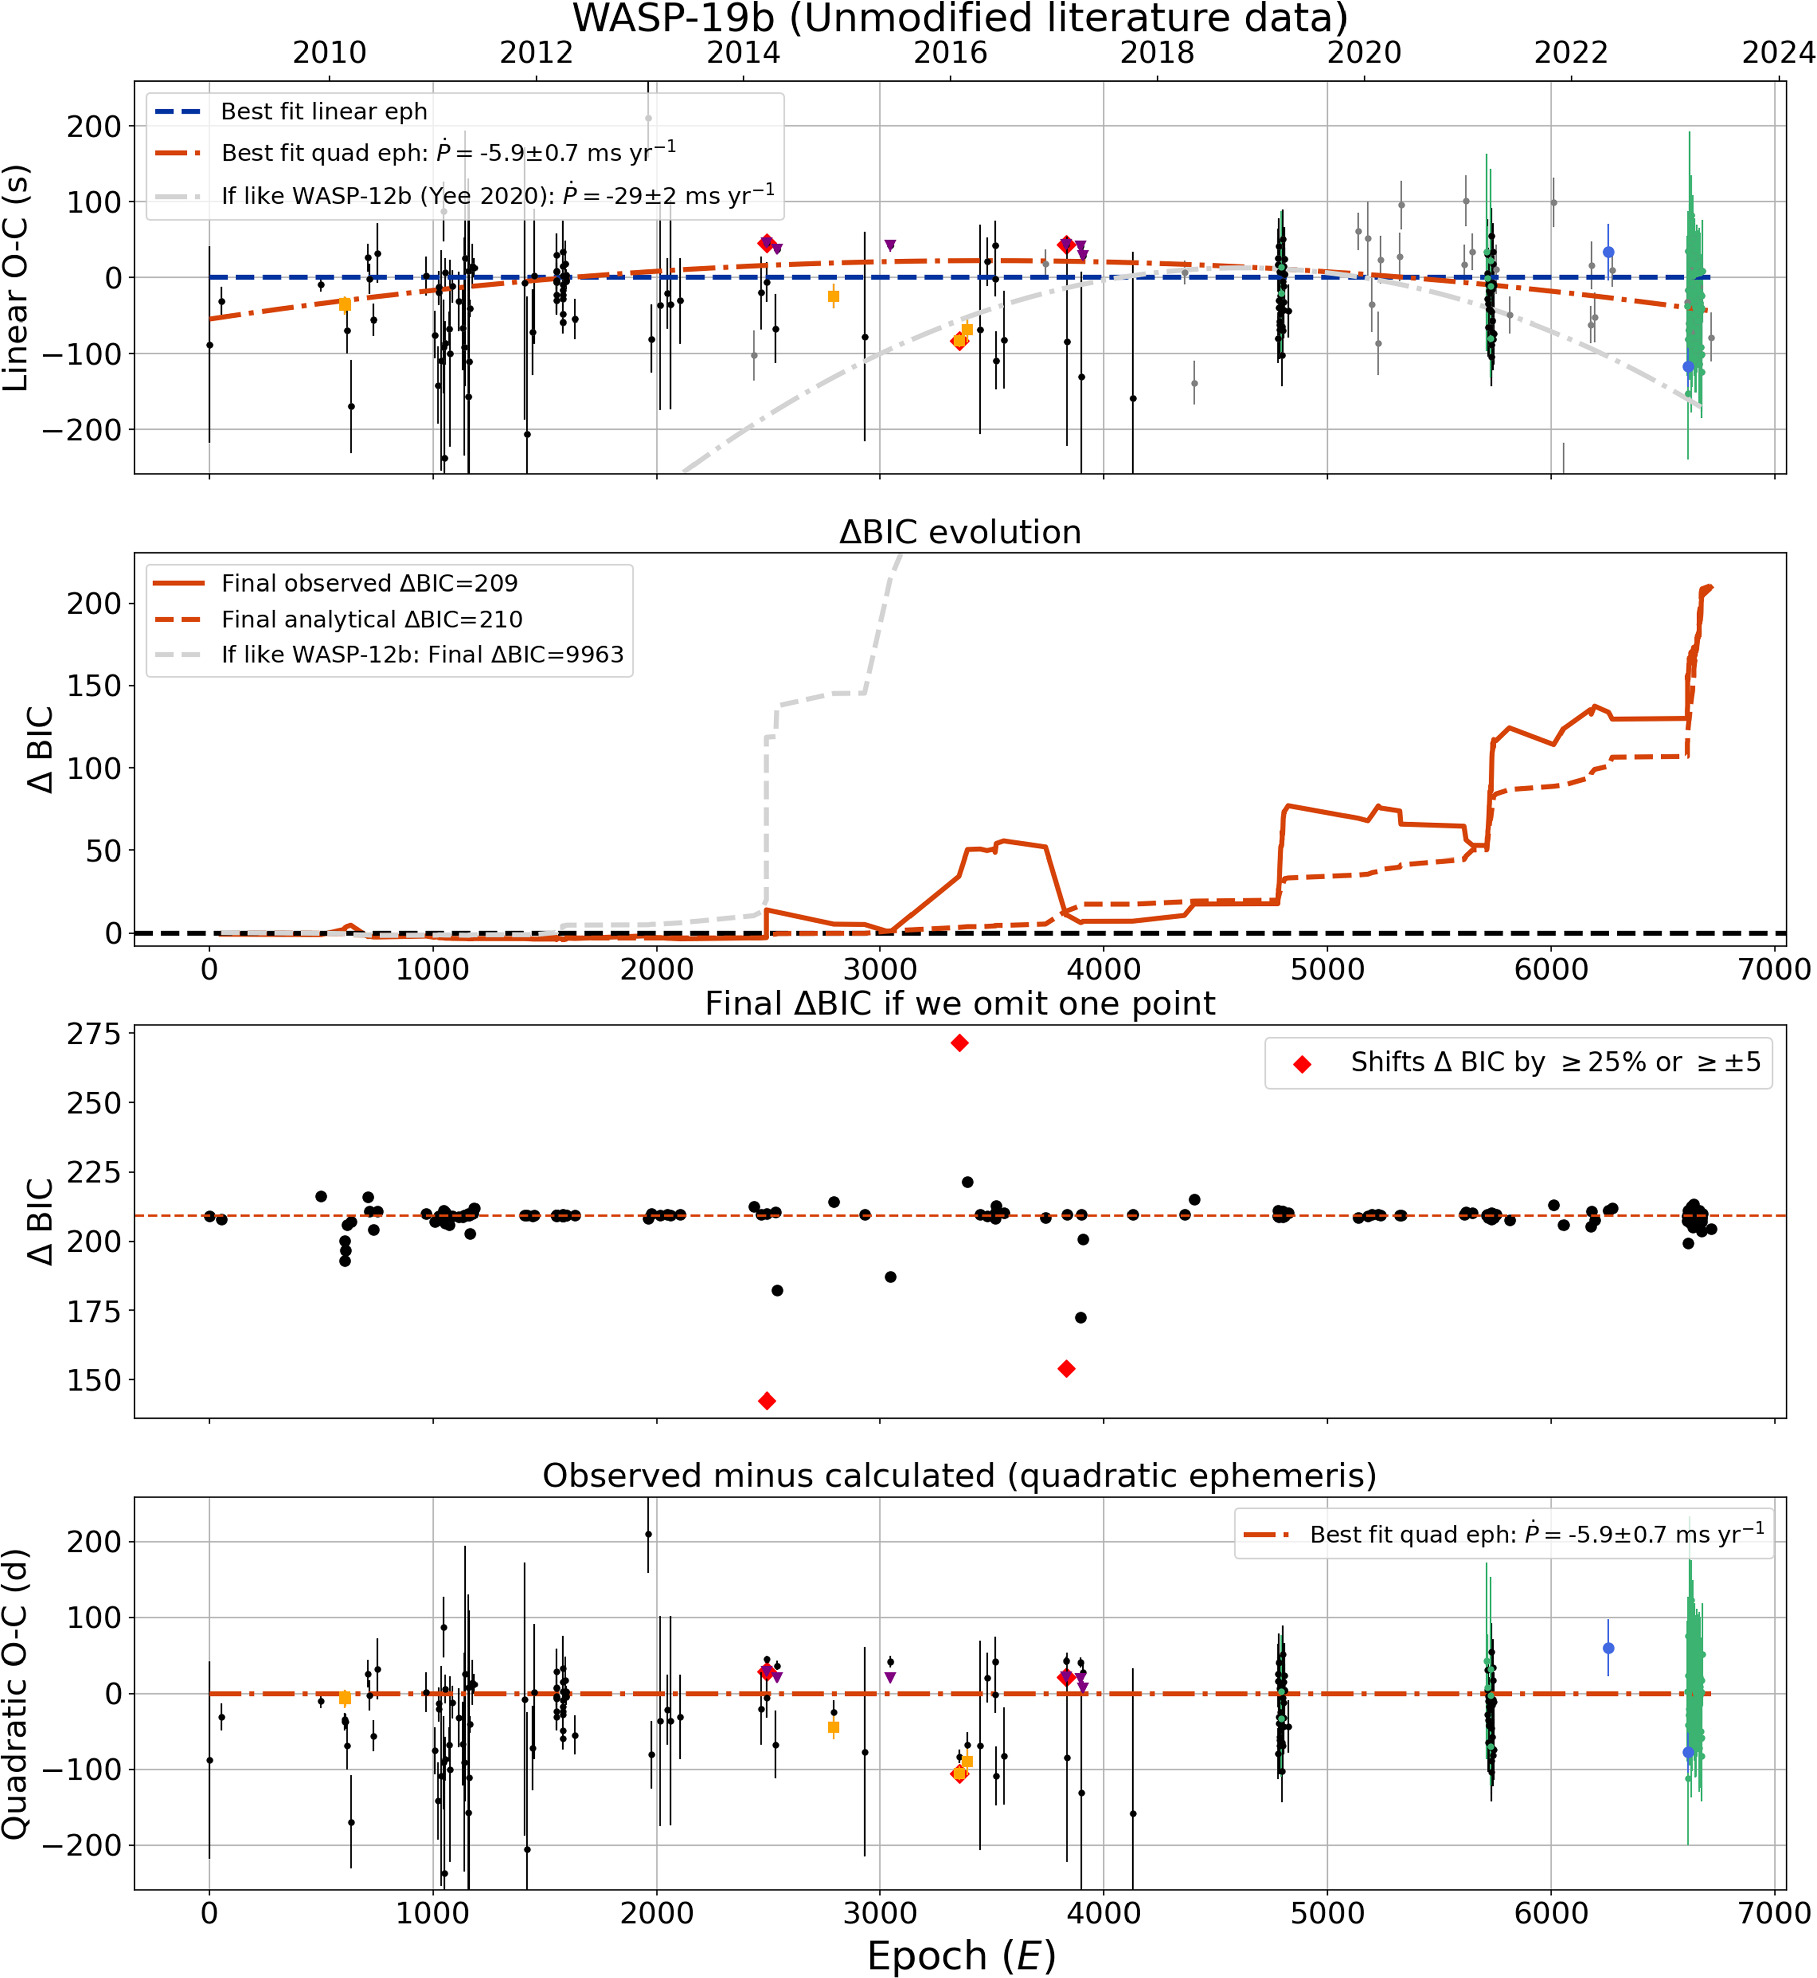
\includegraphics[width=\linewidth]{figs/adams_fig4.jpg}
    \caption{Caption}
    \label{fig:adams-fig4}
\end{figure}

In \ref{fig:adams-fig4}, the data points highlighted by red diamonds have very small error bars compared to the other observations in the data set. These data points greatly affect the value of $\Delta$ BIC, shifting it by 25\% or more when included.

% \subsubsection{Case Study: WASP-12b}
% Discuss the observed orbital decay in WASP-12b, including the measured decrease in transit intervals and its implications. 

% \subsubsection{Long-Term Survey Findings}
% Review the findings of Adams et al. (2024), which reported no new evidence for orbital decay in a long-term survey of 43 UHJs.

% \subsubsection{Discrepancies and Challenges}
% Analyze the discrepancies between different observational studies and the challenges in detecting small changes in orbital periods.





\subsection{Gaps in Current Research}

\subsubsection{Limited Observational Data}
Highlight the need for more extended and precise observational campaigns to detect subtle orbital decay signals.

\subsubsection{Theoretical Model Limitations}
Discuss the limitations of current tidal dissipation models in explaining the varying rates of orbital decay observed.

\subsubsection{Influence of Stellar Properties}
Identify the need for more research on how different stellar properties (e.g., age, rotation rate, magnetic activity) affect tidal dissipation and orbital decay.





\subsection{Proposed Future Research Directions}

\subsubsection{High-Precision Transit Timing}
Advocate for the development of more precise transit timing methods to detect minute changes in orbital periods.

\subsubsection{Comprehensive Surveys}
Propose conducting comprehensive surveys of UHJs with consistent observation protocols to gather uniform data on orbital periods.

\subsubsection{Advanced Modeling}
Encourage the development of more sophisticated models that incorporate a wider range of stellar and planetary properties to predict tidal dissipation and orbital decay more accurately.

- Interpolable grid of values of Q* based on stellar age and mass, so we can redo analytical approximations. For example, figure 1 of Jackson. 





\subsection{Conclusion}

\subsubsection{Summary of Findings}
Recap the key insights gained from synthesizing the five articles on tidal decay in UHJ systems.

\subsubsection{Importance of Continued Research}
Emphasize the significance of addressing the identified research gaps to enhance our understanding of tidal interactions and the evolution of UHJ systems.

\clearpage




\textbf{ADAMS PAPER}

\begin{figure}[htbp]
    \centering
    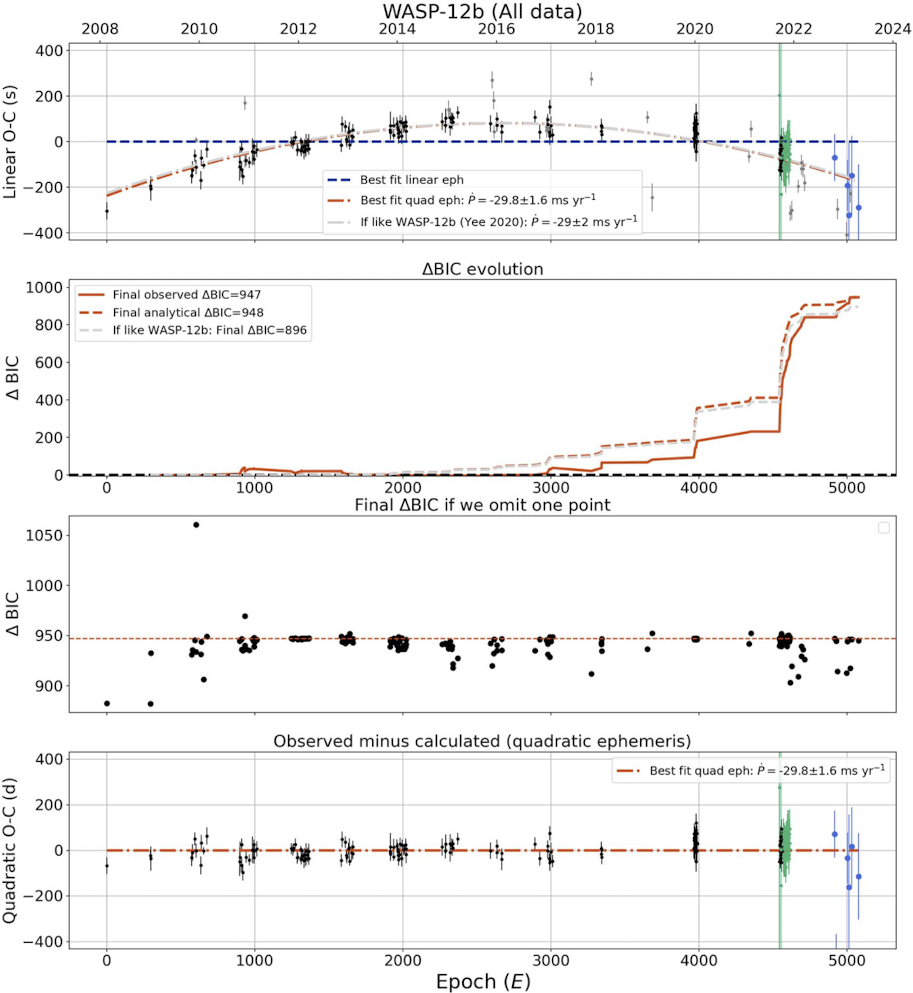
\includegraphics[width=\linewidth]{figs/adams_fig3.png}
    \caption{Caption}
    \label{fig:enter-label}
\end{figure}

\clearpage


\textbf{CARTER PAPER}

\begin{figure}[htbp]
    \centering
    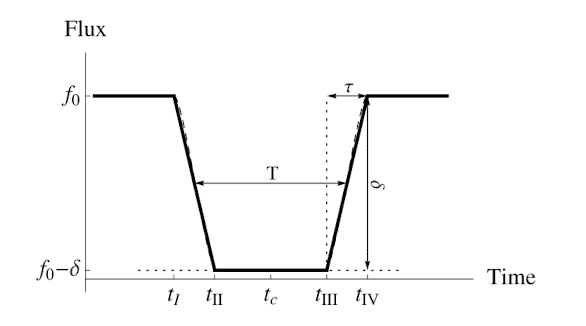
\includegraphics[width=0.5\linewidth]{figs/carter_fig1.png}
    \caption{Caption}
    \label{fig:enter-label}
\end{figure}

\begin{figure}[htbp]
    \centering
    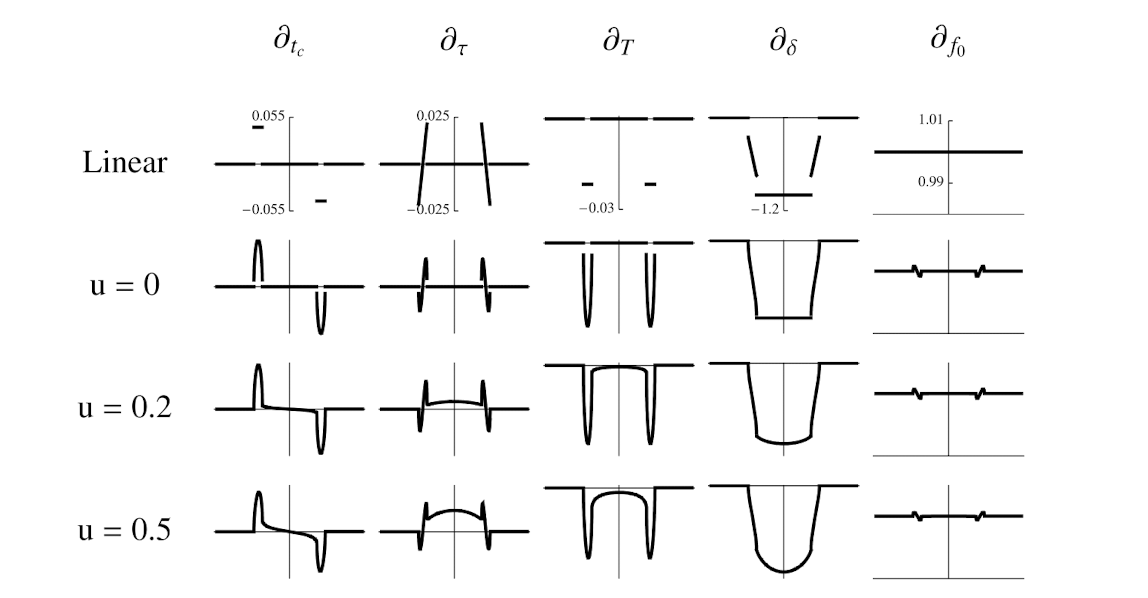
\includegraphics[width=0.5\linewidth]{figs/carter_fig2.png}
    \caption{Caption}
    \label{fig:enter-label}
\end{figure}

\clearpage


\textbf{WINN PAPER}

\begin{figure}
    \centering
    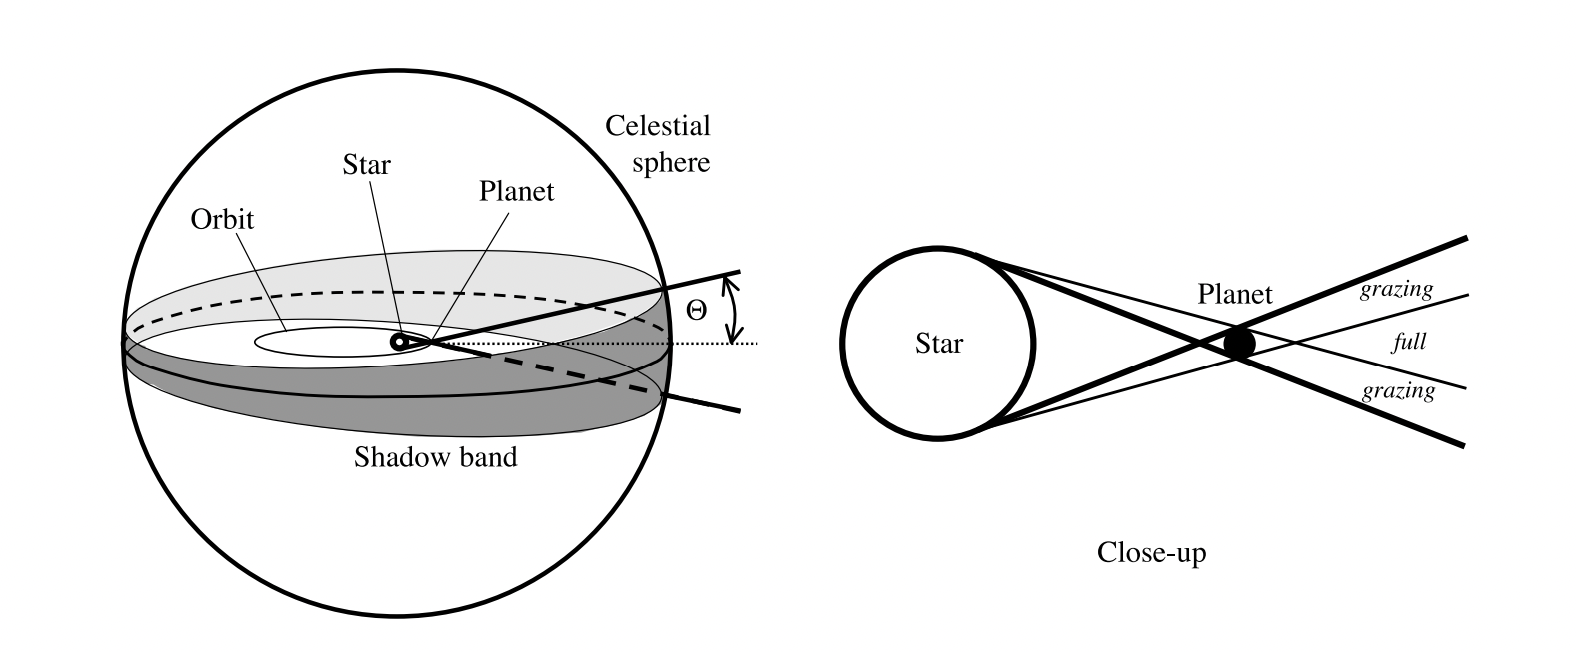
\includegraphics[width=0.5\linewidth]{figs/winn_fig3.png}
    \caption{Caption}
    \label{fig:enter-label}
\end{figure}

\begin{figure}
    \centering
    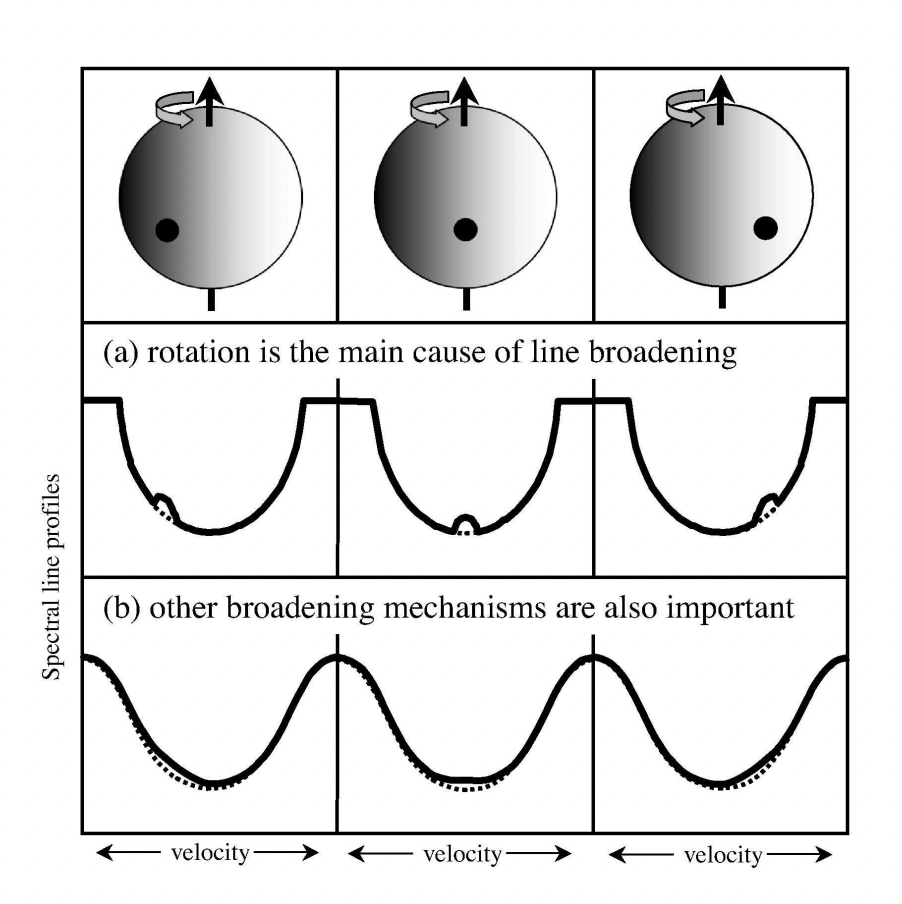
\includegraphics[width=0.5\linewidth]{figs/winn_fig5.png}
    \caption{Caption}
    \label{fig:enter-label}
\end{figure}

\begin{figure}
    \centering
    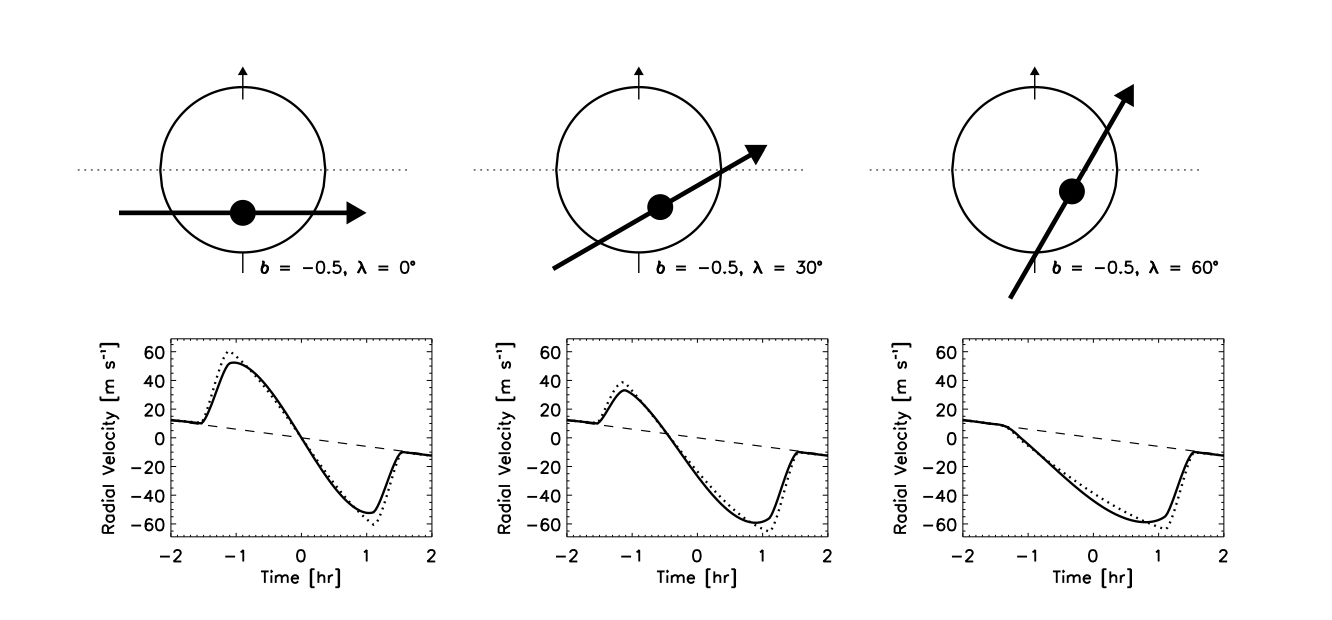
\includegraphics[width=0.5\linewidth]{figs/winn_fig6.png}
    \caption{Caption}
    \label{fig:enter-label}
\end{figure}

\begin{figure}
    \centering
    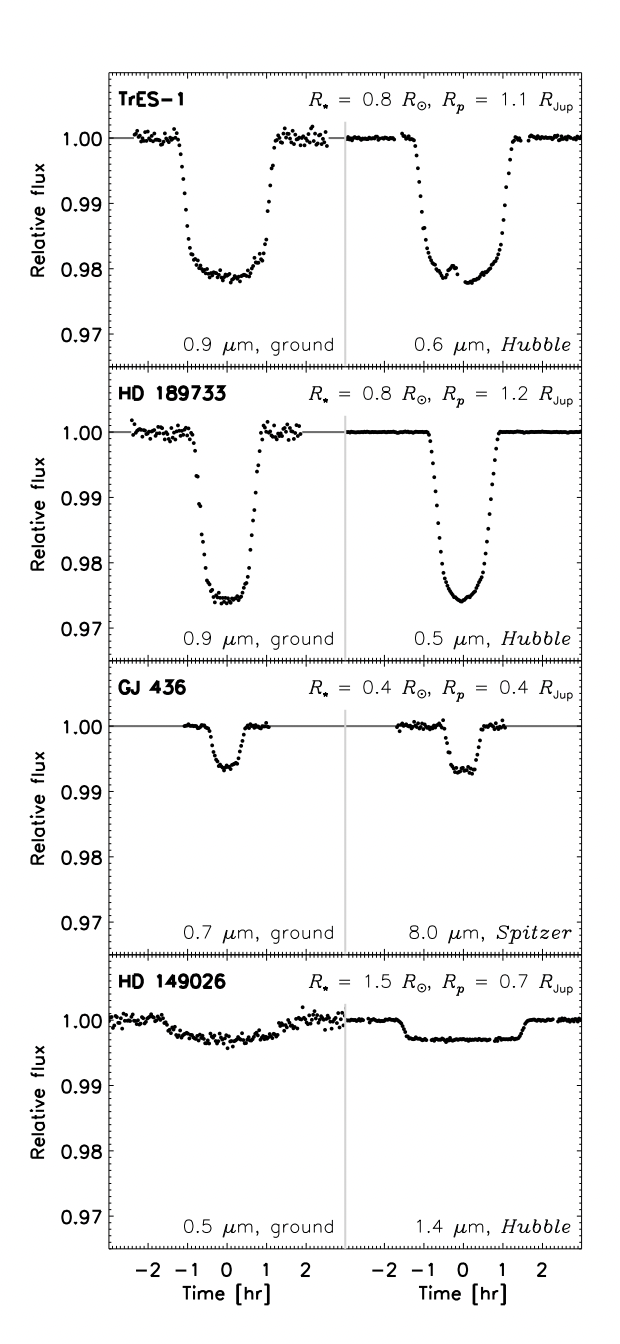
\includegraphics[width=0.5\linewidth]{figs/winn_fig8.png}
    \caption{Caption}
    \label{fig:enter-label}
\end{figure}

\begin{figure}
    \centering
    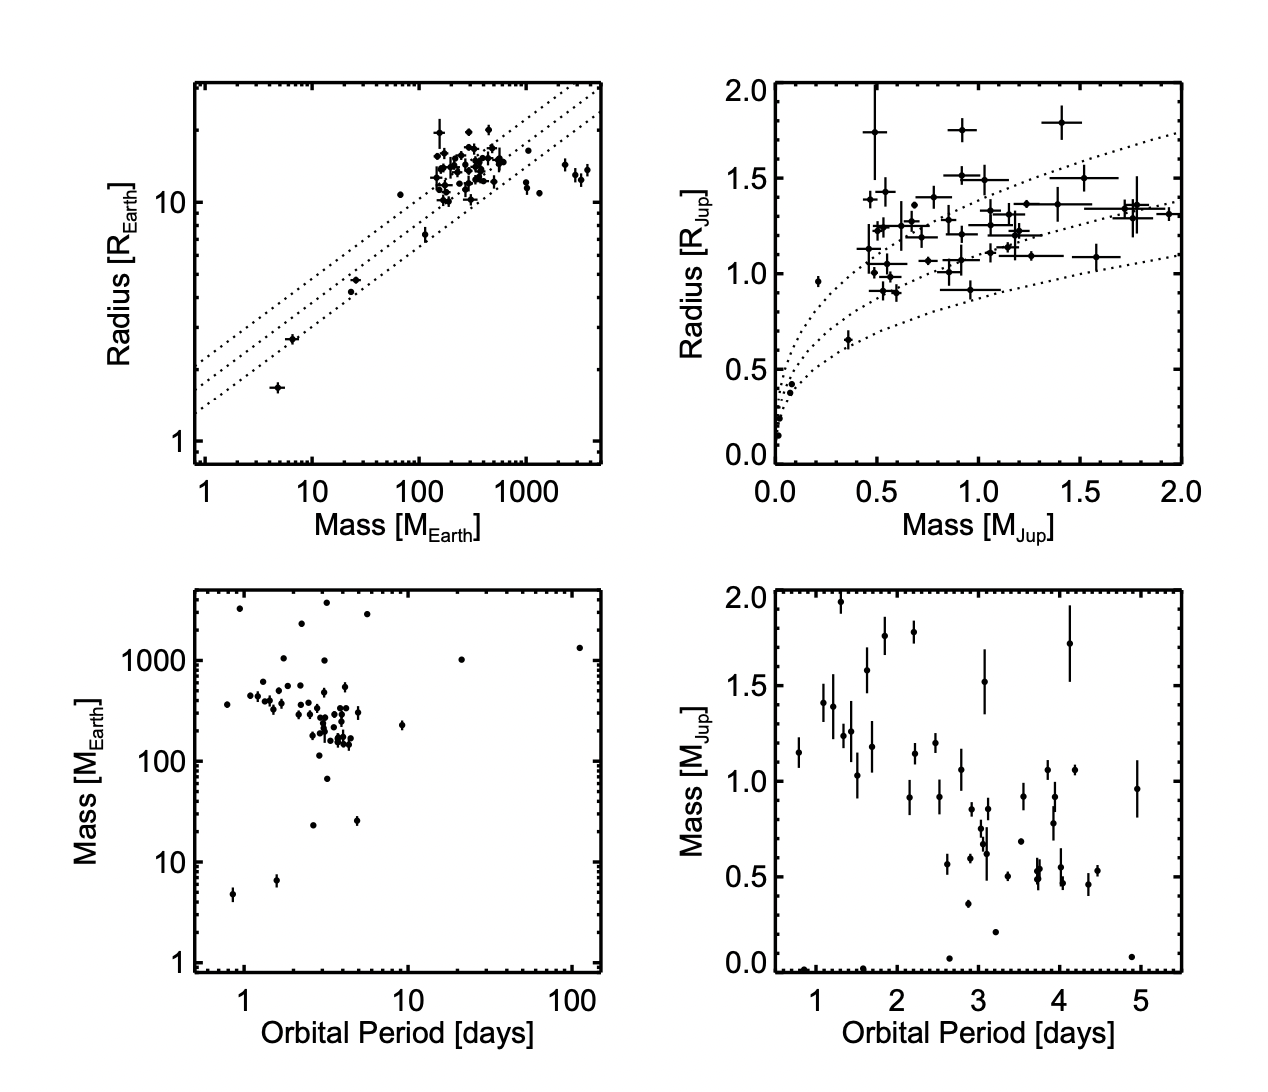
\includegraphics[width=0.5\linewidth]{figs/winn_fig9.png}
    \caption{Caption}
    \label{fig:enter-label}
\end{figure}

\begin{figure}
    \centering
    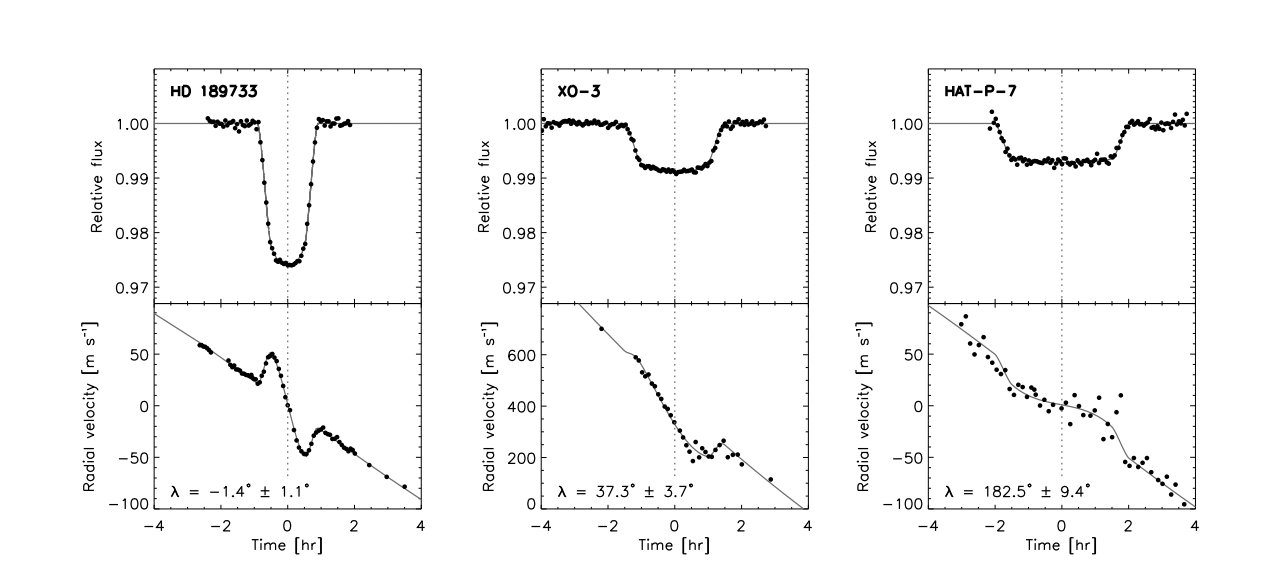
\includegraphics[width=0.5\linewidth]{figs/winn_fig14.png}
    \caption{Caption}
    \label{fig:enter-label}
\end{figure}

\clearpage


\textbf{YEE PAPER}

\begin{figure}[htbp]
    \centering
    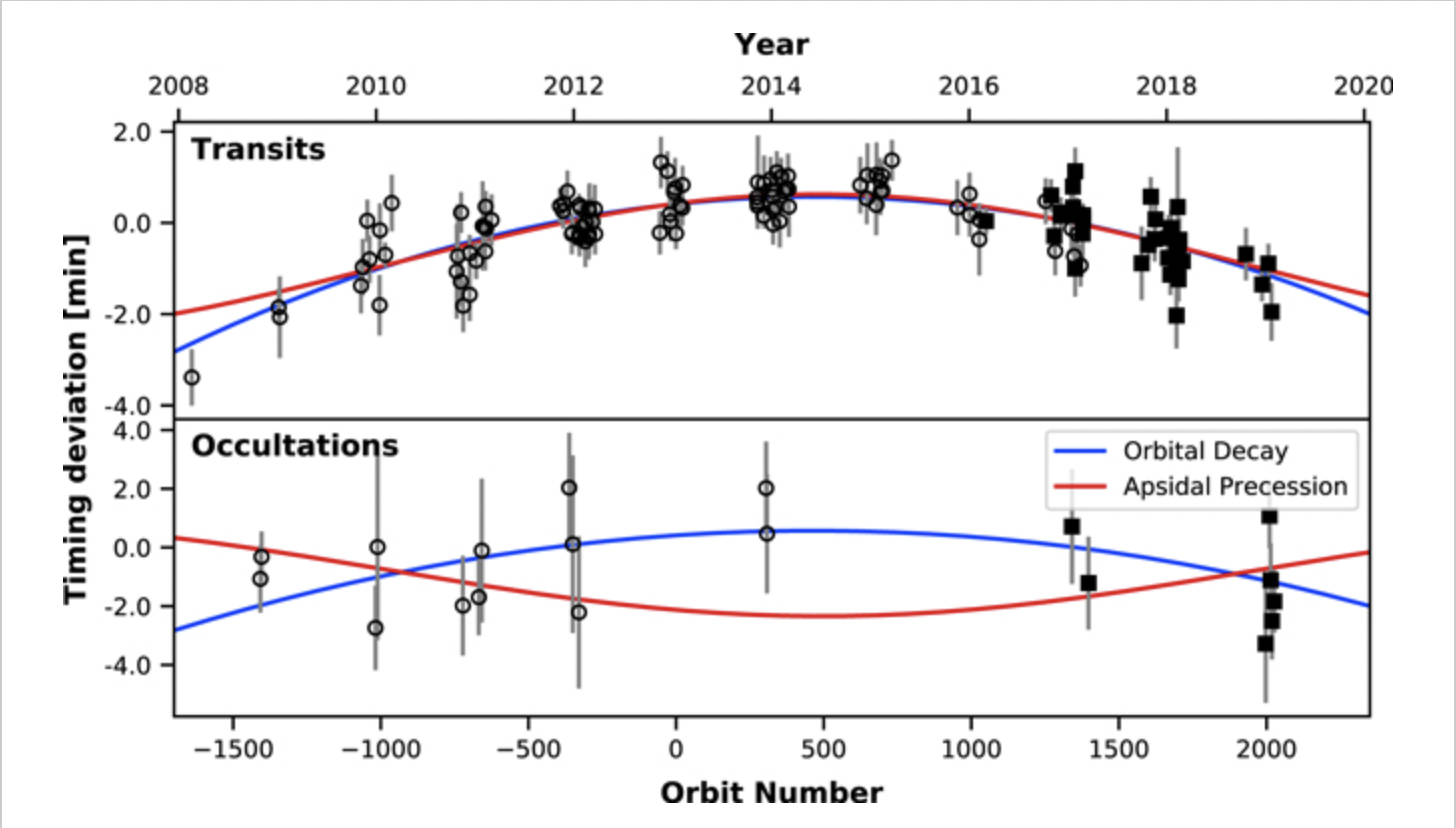
\includegraphics[width=0.5\linewidth]{figs/yee_fig4.png}
    \caption{Caption}
    \label{fig:enter-label}
\end{figure}

\clearpage


PAPER NOTES

% Paper Notes:

% Adams 2024: Doomed Worlds I. No new evidence for orbital decay in a long-term survey of 43 ultra-hot Jupiters
\cite{adams2024doomed}

- UHJs (<3 day orb per) usually occur around younger stars, maybe because something happens to these planets over longer periods of time. This could be planetary engulfment (while stars are still on MS). 
- Q*' gives us estimated planetary engulfment rates, but this is not constrained well. Incorporating NON-linear dissipation (THIS ALSO COMES UP IN OGLIVIE PAPER) has given us a better range depending on stellar age and mass, could be key. 
- With increasing observations over time (a lot now reaching the decade mark) it is easier to start learning trends in the data. However, some systems with limited observations over the years usually are ruled out with additional observations. It is also important to rule out tidal decay by looking at all the other options (apsidal precession, effects of companion objects, line of sight acceleration).
- BIC can help us find optimal observing campaigns because it is obviously important to know how often you need to observe to get optimal results. (THIS CAN TIE INTO BRIAN'S PAPER)
- Some systems, while they show strong evidence for tidal decay, are very difficult to observe from ground based observations and need space-based scopes or largest ground scopes (like Kelper-1658 b)
- Fitting light curves using pylight-curve which uses emcee (by dan). For this work, transit mid-time vals were not sensitive to chosen parameter values such as a/R* or limb-darkening coefficients. WHAT IF IT WAS?? 
- Detection of these timing signatures requires very precise timing analysis. Some issues that have come up with this are detecting duplicate times, composite times, and false timing conversion. This is why it is VERY important to identify exact timing system (to combat false timing conversion) and exact source of the original data (to combat duplicates). 
- Duplicates can have a large impact if it has low errors or occurs at critical point. They are source of error that can be completely eliminated with proper data maintenance.
- Composites (times derived from more than 1 light curve) can have the following issues: their error bars are usually much smaller because they compress all timing info into single point, they obscure original data source which makes it difficult to find potential timing errors, and can lead to double counting transits
     - Composited include the following: stacked light curves where transits from multiples epochs are stacked to actually see the transits, which is common in ground-based surveys where it is difficult to detect a single transit; when ephemeris mid-times are reported for composite data, this usually anchors all the combined transits into one reported epoch, which results in a very specific (small error) mid-time for one epoch and will weight the BIC equation; weighted average times are when two mid-times from different sources are averaged together, which makes it difficult to deconstruct this and look for errors in the observations
     - Example of a composite mid-time is for CoRoT-2 where 82 transits were stacked and when unstacked, the original transits had 50 percent larger errors, which changed delta BIC from 33 to -2 (pretty much ruling out tidal decay)
- Timing systems: 
    - to remove the motion of the earth around the sun and the motion of the sun around the solar system barycenter, we must use a dynamical timing system to avoid cyclical variations in astronomical time series. This is why we use BJD TDB timing system and scale (respectively). 
    - Historically, helicentric julian date HJD is much easier to calculate and this has been preferred over BJD, and one can argue that using one or the other doesn't have much significance as the difference is only about 1 second and most transit observations do not have the accuracy within this range to be affected. However, HJD is usually in UTC time scale while BJD is usually in TDB timescale. This difference is about 64.184 seconds as of 2024 (this offset changes with addition of leap seconds). This is why it is very important to also report the time SCALE as well as the system, which isn't always reported and more often than not assumed to be associated (UTC with HJD, TDB with BJD). 
- Running models: fit to linear and quadratic models, calculated delta BIC, ran omit-one delta BIC test, calculated a rescaled delta BIC, investigated outliers that failed the omit one test and re-ran everything again with corrected data
- Timing Analysis: 
    - WASP-12 b: still looking good
    - WASP-19 b: period of just 0.79 days and data spanning 15 yrs (good candidate), however, decaying at an order of magnitude smaller than 12b which makes Q*' an order of magnitude larger, however, timing errors that were corrected made the delta BIC drop to insignificant levels, this may be ruled out as candidate
    - CoRoT-2 b: Data spanning 18 yrs, had composite errors (in CoRoT mission data, 82 transits were combined), timing scale errors (in ETD, data was labeled as HJD when it was really JD and in a Ozturk&Erdem, data was labeled as BJD/TDB but was possibly JD), and duplicate errors. Once all of these errors were addressed, the results delta BIC was -2, showing no tidal decay
    - WASP-121 b: the early data really need to be refit but the actual timing data has not been published, so this cannot happen. When scaled, the delta BIC still stayed positive (14), showing that the error bars are good and this system just really needs more data observed
    - WASP-46 b: Has good data, lots of scatter in data before 2015 with 7 outlier points, removing these points changes delta BIC from 32-149, and when rescaled changes to 2, flagged for reanalysis
    - TrES-1 b: good baseline of data and no obvious timing errors, has siginifgant positive delta BIC (69) HOWEVER, the Q*' value is five orders of magnitude lower than what we expect for the decay rate, so the decay is most likely caused by something else
    - Kepler-1658 b: has a very shallow transit depth, so hard to observe with ground-based telescopes. rapidly decaying and star is evolved off MS, weinburg says g-mode does not explain rapid decay but vissapragada says could be inertial wave dissipation and rapid stellar rotation. confirmation could be possible with a few more observations, so withing a year or two
- Answering the question: was WASP-12 b the first world to have detected tidal decay because it had enough transits observed OR is there something special about the WASP-12 b system?
    - Test 1: Sets all planet's decay rates to WASP-12 b decay rate and sees what the delta BIC would be given the number of observations each system has. Shows that nearly half of the systems would have has delta BIC > 30 (in reality only 1 did) and 4 systems would have had 10x larger delta BICS than WASP-12b
    - Test 2: Sets Q*' (tidal dissipation factor) to be the same for all systems and calculated the decay rate for each system. seven planets had value >= 3x the observed error in the decay rate
    - Overall, for 20 of the systems, there is evidence that we should have detected tidal decay but we have not
- Calculated values of Q*' (tidal dissipation factor) and tau (estimate decay timescale). Q*' is inversely proportional to rate of period change. 
- Weinberg 2024 has table of Q*' based on stellar age and mass that can be interpolated. Stellar models with radiative cores and convective envelopes usually have smaller values than higher mass MS stars with convective cores. If highmass stars are not on the MS, then they no longer have a convective (instead, radiative) core and the Q*' value drops again. CAN TIE THIS INTO OGLIVIE PAPER
- CONCLUSIONS: 
    - For the two systems where orbital decay is likely (WASP-12 b and Kepler-1658 b), their host stars may have evolved off the MS which would offer explanation for rapid decay and maybe point towards evidence that a star needs to be evolved off the MS to exhibit decay (QUESTION: but then what does that say about the observation that most UHJ are around young stars?)
    - delta BIC values below 30-50 should be tentative because of usual timing data errors, especially in the estimation of timing uncertainties
    - systems need to be observed at least once a year
    
% Jackson 2023: Metrics for Optimizing Searches for Tidally Decaying Exoplanets
\cite{jackson2023metrics}

- For host stars rotating more slowly than the planet, interaction between planet and tidal bulge transfers angular momentum from the planet's orbit to the star (this can tie into OGLIVIE PAPER)
- Stellar dissipation rate may be related to stellar luminosity
- Once gas giant spirals into roche limit, tidal disruption can occur
    - Stable: decay timescale determined by tidal decay rate
    - UNstable: disruption proceeds rapidly
    - Direct accretion if roche limit lies within star
- Signs of tidal disruption: tidal/accretion-induced spin-up, young MS stars, anomalous chem signatures in red giants that may be caused by planetary engulfment (maybe in MS stars as well)
- based on Q*' (which this scales with it), planetary engulfment occurs between 0.1 and 1/year in milky way HOWEVER, the value of Q*' may not be set and may depend on a few things (CAN TIE THIS INTO OTHER PAPERS), ONE WAY to constrain this observationally (and not theoretically with stellar models) is to observe tidal decay
- Based on Carter 2008 equations, we get equation 11, the uncertainty on the central time (QUESTION: is this mid-time?), which shows that the uncertainty increases with photometric uncertainty, decreases as transit depth and sampling rate increase. Also increases with ingress/egress duration because if b->1 (very long ingress/egress) then the light curve would be nearly v-shaped and we would need the exact time it switches from a downwards trend to an upwards trend to get the mid-time accurately
- Figure 1 shows possible mid-time uncertainties on some systems based on equation 12, which relates uncertainty to stellar magnitude
- We can use equation 18 to calculate the time at which the uncertainty on the transit becomes larger than the transit duration. Figure 3 shows some systems with their critical point of the uncertainty growing larger than transit duration and time that has passed since its last observation. Anything below the y=x line is something that has maybe passed the point of uncertainty being larger than transit duration and thus would be useful to follow up on
- Equation 22 predicts the orbital decay rate (dP/dE) based on stellar and planetary parameters. HOWEVER, applications in the paper use a constant fixed value of Q*, which isn't exactly true (can tie into Ogilvie paper)
- Note: in figure 4, there is a S/N which means signal to noise, which is just the "signal" or the actual decay rate divided by the "noise" or the uncertainty.
- Because dP/dE is so much smaller than T0 and P, T0 and P need to have pretty small error bars to be able to say we see an actual dP/dE signal
- We can use equation 35 to estimate expected delta BIC for future observations
- As we can see in figure 6, delta BIC initially decreases, showing preference for linear model, before increasing. This is because curvature needs to build up over time to see the quadratic term. Depending on the number and frequency of observations, timing uncertainties, and decay rate, we can calculate the crossover epoch, which is the point at which a quadratic model is favored over a linear model. For example, we can choose a desired delta BIC and assign system properties (dP/dE, timing uncertainties) and calculate the minimum number of transits observed before crossover epoch is achieved. So, we can apply this equation to a number of different observing campaign goals and get some info back
- Overall, can use the analytical delta BIC equation to plan different observing campaigns and see best way to collect data in not only frequency and total number, but also with uncertainties based on ground and space-based scopes (CAN TIE THIS INTO UNCERTAINTIES MAYBE?)
- Section 3.2 shows real analysis of analytical delta BIC application for 4 different planetary systems. Shows that these systems will not usually reach WASP-12 b levels of delta BIC decay detection until 2030 (TrES-1 b), 2025 (TrES-2 b), 2024 (HAT-P-19 b, although this one is super weird, maybe because of uncertainties??)
- Caveats: 
    - used a linear regression approach for the uncertainties (the whole S thing from numerical recipes) and thus analytical delta BIC equation, but real data could have asymmetric uncertainties (QUESTION: is this what Brian is usually talking about when he mentions gaussian uncertainties??)
    - delta BIC usually only works when sample size is much larger than the number of model parameters (however this is usually fulfilled because to search for decay you need a lot of observations anyways)
    - doesn't look into precession and/or other forms of changing orbit

% Carter 2008: Analytical Approximations for Transit Light-Curve Observables, Uncertainties, and Covariances 
\cite{carter2008analytic}

- light curves can be used to find planet parameters, this uses an analytical approach to estimate these parameters without light curves?
- transit light curves can tell us about planetary and stellar radii, orbital inclination, and mean density of the star. Can also detect other planets in system by observing changes in orbital params or changes in collections of mid-times
- Even when it is possible to have numerical values, it can help to have analytical approximations as well as uncertainties and covariances
- Analytical apprx are good for:
    - Planning observations. For example: which systems will have most precise measurement of orbital inclination, how many transits do I need to observe before stat error in planetary radius is smaller than systematic err
    - Speeding up convergence of optimization algos
    - useful in order-of-mag estimates of observability of subtle transit effects such as: TTVs, precession-induced changes, asymmetry in ingress and egress due to non-zero eccentricity
- Their models assume flux measurements are made continuously throughout transit and stellar limb darkening is neglible
- Approximation of no limb darkening can ACTUALLY be used for mid-IR bandpasses (WHY??) so everything in this paper assumes observations around the IR bandpasses so that limb darkening effects can be ignored
- Equation 1 and 2 are exact solutions, to make more analytical approximations, some assumptions are made:
    - assume orbital period is large compared to transit duration
    - assumes transit occurs in a uniform, straight line motion across stellar disk (meaning it has constant velocity, QUESTION: what would it look like if it didn't? is this something worth discussing?)
- Equation 3 is analytical approximation given the above assumptions
- Equations 4 and 5 are analytical approximations of two characteristic timescales, time between ingress and egress midpoints and total "ingress" time
- These equations can be expanded to include eccentric orbits by replacing a (semimajor axis) and n (angular frequency)
- Equations 8-11 are for a piecewise "linear in time" model light curve denoted as F1
    - Deviation in this approximation occur near ingress and egress phases (QUESTION: is this because this is linear piecewise function?)
    - Most accurate for small values of r & b
    - Least accurate for grazing transits
- Uses Fisher information analysis to find correlation between parameters (there are 5 in the model: t_c (time of conjunction), tau (QUESTION: what exactly is tau on pg 2), T (total transit time?), delta (idk), and f_0 (unocculted flux)
    - When you look at partial time derivative of each parameter, you can see that the model reflects the symmetry of the "real" behavior
    - t_c is uncorrelated with the other params
- Equation 20 is the covariance matrix for the piecewise function
- Equation 21 is the covariance matrix for the piecewise function if we assume we have a great baseline of the unocculted flux f_0 so that f_0=1, making delta the fractional transit depth
    - From this we can see that theta is the key controlling param, where theta = r/(1-b^2)


% Ogilivie 2014: Tidal dissipation in stars and giant planets
\cite{ogilvie2014tidal}

- 

% Winn 2010: Transits and Occultations
\cite{winn2010transits}

- 

% TODO
- Look more into line-of-sight acceleration
- Should I fully understand the observatory information (example: IoIo info pg 3 of elisabeths' ppr)
- What does it mean by observations were mostly taken in R?
- Limb-darkening coefficients? (brought up in Adams and Jackson)
- Composite times?
- Rescaled delta BIC from Adams? Obviously this is important and something I will definitely need to touch on when discussing associated  mid-time errors in timing observations/processing sections 
- What could a period increase mean?
- Don't fully understand the 2 tests ran on pg 25 of adams
- Don't fully understand the Q*' thing at the end (pg 25/26)
- Stellar dissipation rate may be related to stellar luminosity?

\clearpage

\section{References}
\printbibliography[heading=none]
\end{document}